\documentclass[10pt]{oden_beamer}
%Information to be included in the title page:
\title{Numerical Simulation of Compound Flooding using Parametric Rainfall Models}
\author{Chayanon (Namo) Wichitrnithed \inst{1}, Eirik Valseth \inst{1}, Younghun Kang \inst{2}, Mackenzie Hudson \inst{2}, Ethan Kubatko \inst{2}, Clint Dawson \inst{1}}
\institute{\inst{1} Computational Hydraulics Group, University of Texas at Austin \\ \inst{2} Computational Hydrodynamics and Informatics Lab, Ohio State University}
\date{November 2022}

\usepackage{caption}
\usepackage{xurl}
\usepackage{soul}

%\usetheme{Madrid}
\newcommand\dt[1]{\frac{\partial #1}{\partial t}}
\newcommand\Dt[1]{\frac{d #1}{dt}}
\newcommand\dx[1]{\frac{\partial #1}{\partial x}}
\newcommand\dy[1]{\frac{\partial #1}{\partial y}}

\begin{document}

\frame{\titlepage}

\begin{frame}
\frametitle{Motivation}
\begin{columns}
  \column{0.5\linewidth}
\begin{itemize}
\item Compound flooding - a high-impact, simultaneous interaction between multiple sources
  \begin{itemize}
  \item Storm surge from the ocean
  \item River discharge
  \item Rainfall
  \end{itemize}
\item Example: Hurricane Harvey (2017) - storm surge blocked drainage of rainfall runoff and amplified inundation
\item Difficult to model due to the nonlinear nature of the interaction; no single model encompasses all flooding sources
\end{itemize}

  \column{0.5\linewidth}
  \begin{figure}[h]
    \centering
    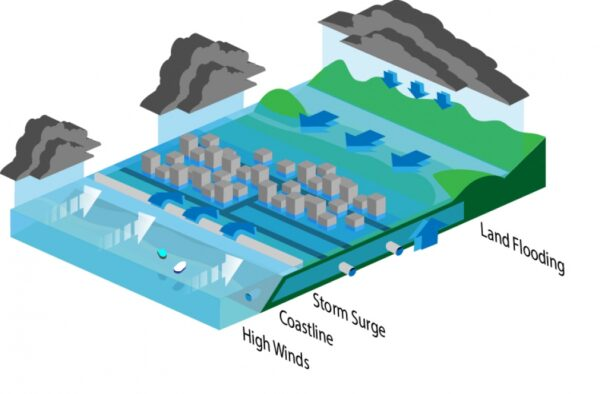
\includegraphics[width=\linewidth]{compound.jpg}
  \end{figure}
    \tiny Image from \url{http://sites.utexas.edu/climatesecurity/2020/03/25/flooding-from-all-directions-how-compound-flooding-threatens-urban-areas-in-oceania/}
\end{columns}
\end{frame}

\begin{frame}
  \frametitle{}
  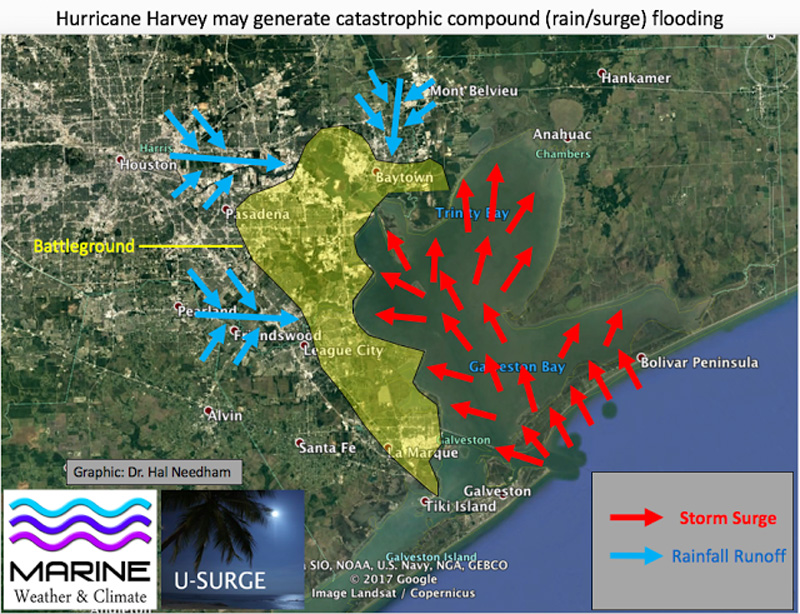
\includegraphics[width=0.9\linewidth]{houston.jpg} \\
  \footnotesize
  Image from U-Surge. \url{https://wxshift.com/news/blog/harveys-rain-and-surge-flooding-could-be-catastrophic}
\end{frame}

\begin{frame}
  \frametitle{Computational Difficulties}
  \begin{itemize}
  \item Advanced Circulation model (ADCIRC) (Luettich and Westerink, 2004). Galerkin finite element program that simulates coastal storm surge given wind input
  \item Runoff effects can be added to ADCIRC via flux boundary conditions from gauge data
  \item Difficulty adding direct rainfall on ADCIRC due to the form of the equation and possibly the continuous Galerkin method
  \item This work: adding rainfall to the Discontinuous Galerkin Shallow Water Equation Model (DG-SWEM) (Kubatko, 2006) based on ADCIRC
  \end{itemize}
\end{frame}

\begin{frame}
  \frametitle{Mathematical Model}
  \centering
  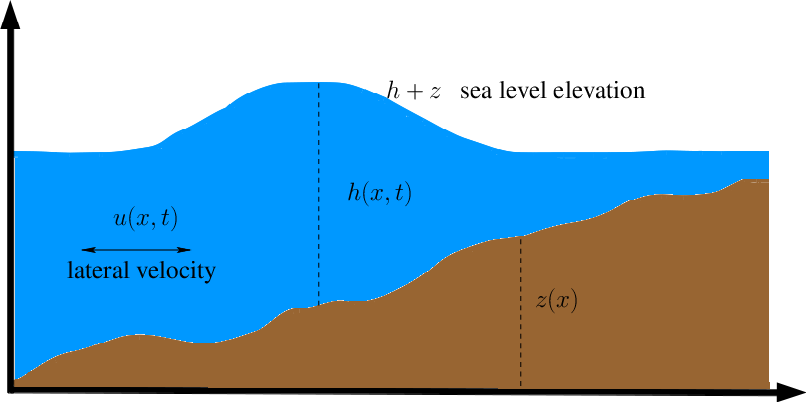
\includegraphics[width=0.9\textwidth]{shallow.png} \\
  \footnotesize Diagram from H. Gunawan.
\end{frame}

\begin{frame}
  \frametitle{Mathematical Model}
  Assuming depth is small relative to horizontal scale, we can average over the z-direction to obtain
  \begin{block}{The Shallow Water Equations}
    \begin{align*}
      \dt{\zeta} + \dx{(Hu)} + \dy{(Hv)}  &= \textcolor{red}{S(t,x,y)} \\
      \dt{(Hu)} + \dx{(Hu^2+\frac{1}{2}g(H^2-h^2))} + \dy{(Huv)} &= g\zeta\dx{h} + F_x \\
      \dt{(Hv)} + \dx{(Huv)} + \dy{(Hv^2+\frac{1}{2}g(H^2-h^2))} &= g\zeta\dy{h} + F_y
    \end{align*}
  \end{block}
  where \\
  $\zeta =$ surface elevation \\
  $H = $ total depth, $h = $ bathymetric depth \\
  $u,v = $ depth-averaged horizontal velocities \\
  $F_x,F_y = $ horizontal forces including friction \\
  $\textcolor{red}{S} = $ source/sink term
\end{frame}

\begin{frame}
  \frametitle{Compact Form of the Equations}
  Rewriting terms into matrix/vector form  gives
  \begin{block}{The Shallow Water Equations (conservation form)}
    \begin{align*}
    \dt{\mathbf{w}} + \nabla \cdot \mathbf{F}(\mathbf{w}) = \mathbf{r}(\mathbf{w})
    \end{align*}
  \end{block}
  where
  \begin{align*}
    \mathbf{w} &=
                 \begin{bmatrix}
                 \zeta, & uH, & vH
                 \end{bmatrix}^T \\
    \mathbf{r} &=
                 \begin{bmatrix}
                   \textcolor{red}{S}, & gH\dx{\zeta} + F_x,  & gH\dy{\zeta} + F_y
                 \end{bmatrix}^T \\
    \mathbf{F} &=
                 \begin{bmatrix}
                   uH & vH \\
                   Hu^2 + g(H^2-h^2) & Huv \\
                   Huv & Hv^2 + g(H^2-h^2)
                 \end{bmatrix}
  \end{align*}
\end{frame}

\begin{frame}
  \frametitle{Discretization}
  \begin{itemize}
  \item DG-SWEM uses the discontinuous Galerkin (DG) method to discretize in space and Runge-Kutta in time
  \item Combines advantages of FEM and FVM:
    \begin{itemize}
    \item Finite element: high-order basis functions, works well on complex geometries
    \item Finite volume: designed for conservation laws, guarantees local mass conservation, stability achieved from numerical flux
    \end{itemize}
  \end{itemize}
  \begin{figure}[h]
    \centering
    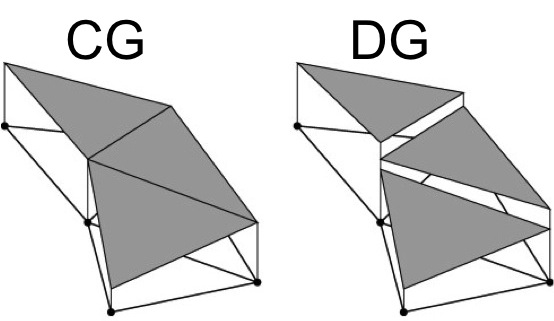
\includegraphics[width=0.5\textwidth]{cgdg.jpg}
    \caption*{Image from \url{https://mathstats.uncg.edu/applied/dgfiniteelement/}}
  \end{figure}
\end{frame}

\begin{frame}
  \frametitle{Computational process in each timestep}
  \begin{enumerate}
  \item  State variables at timestep $n$
    \begin{align}
      \mathbf{w}^n = [\zeta^{(n)}, uH^n, vH^n]
    \end{align}
  \item Discretize in space using DG to get
    \begin{align}
        \Dt{\mathbf{w}^n} = L_h(\mathbf{w}^n)
    \end{align}
  \item Step in time using SSP Runge-Kutta to get
      $\mathbf{w}^{(n+1)}$
  \item Average the solution on each node
  \end{enumerate}
\end{frame}
\begin{frame}
  \frametitle{Computational Domain}
  \begin{figure}[t]
    \centering
    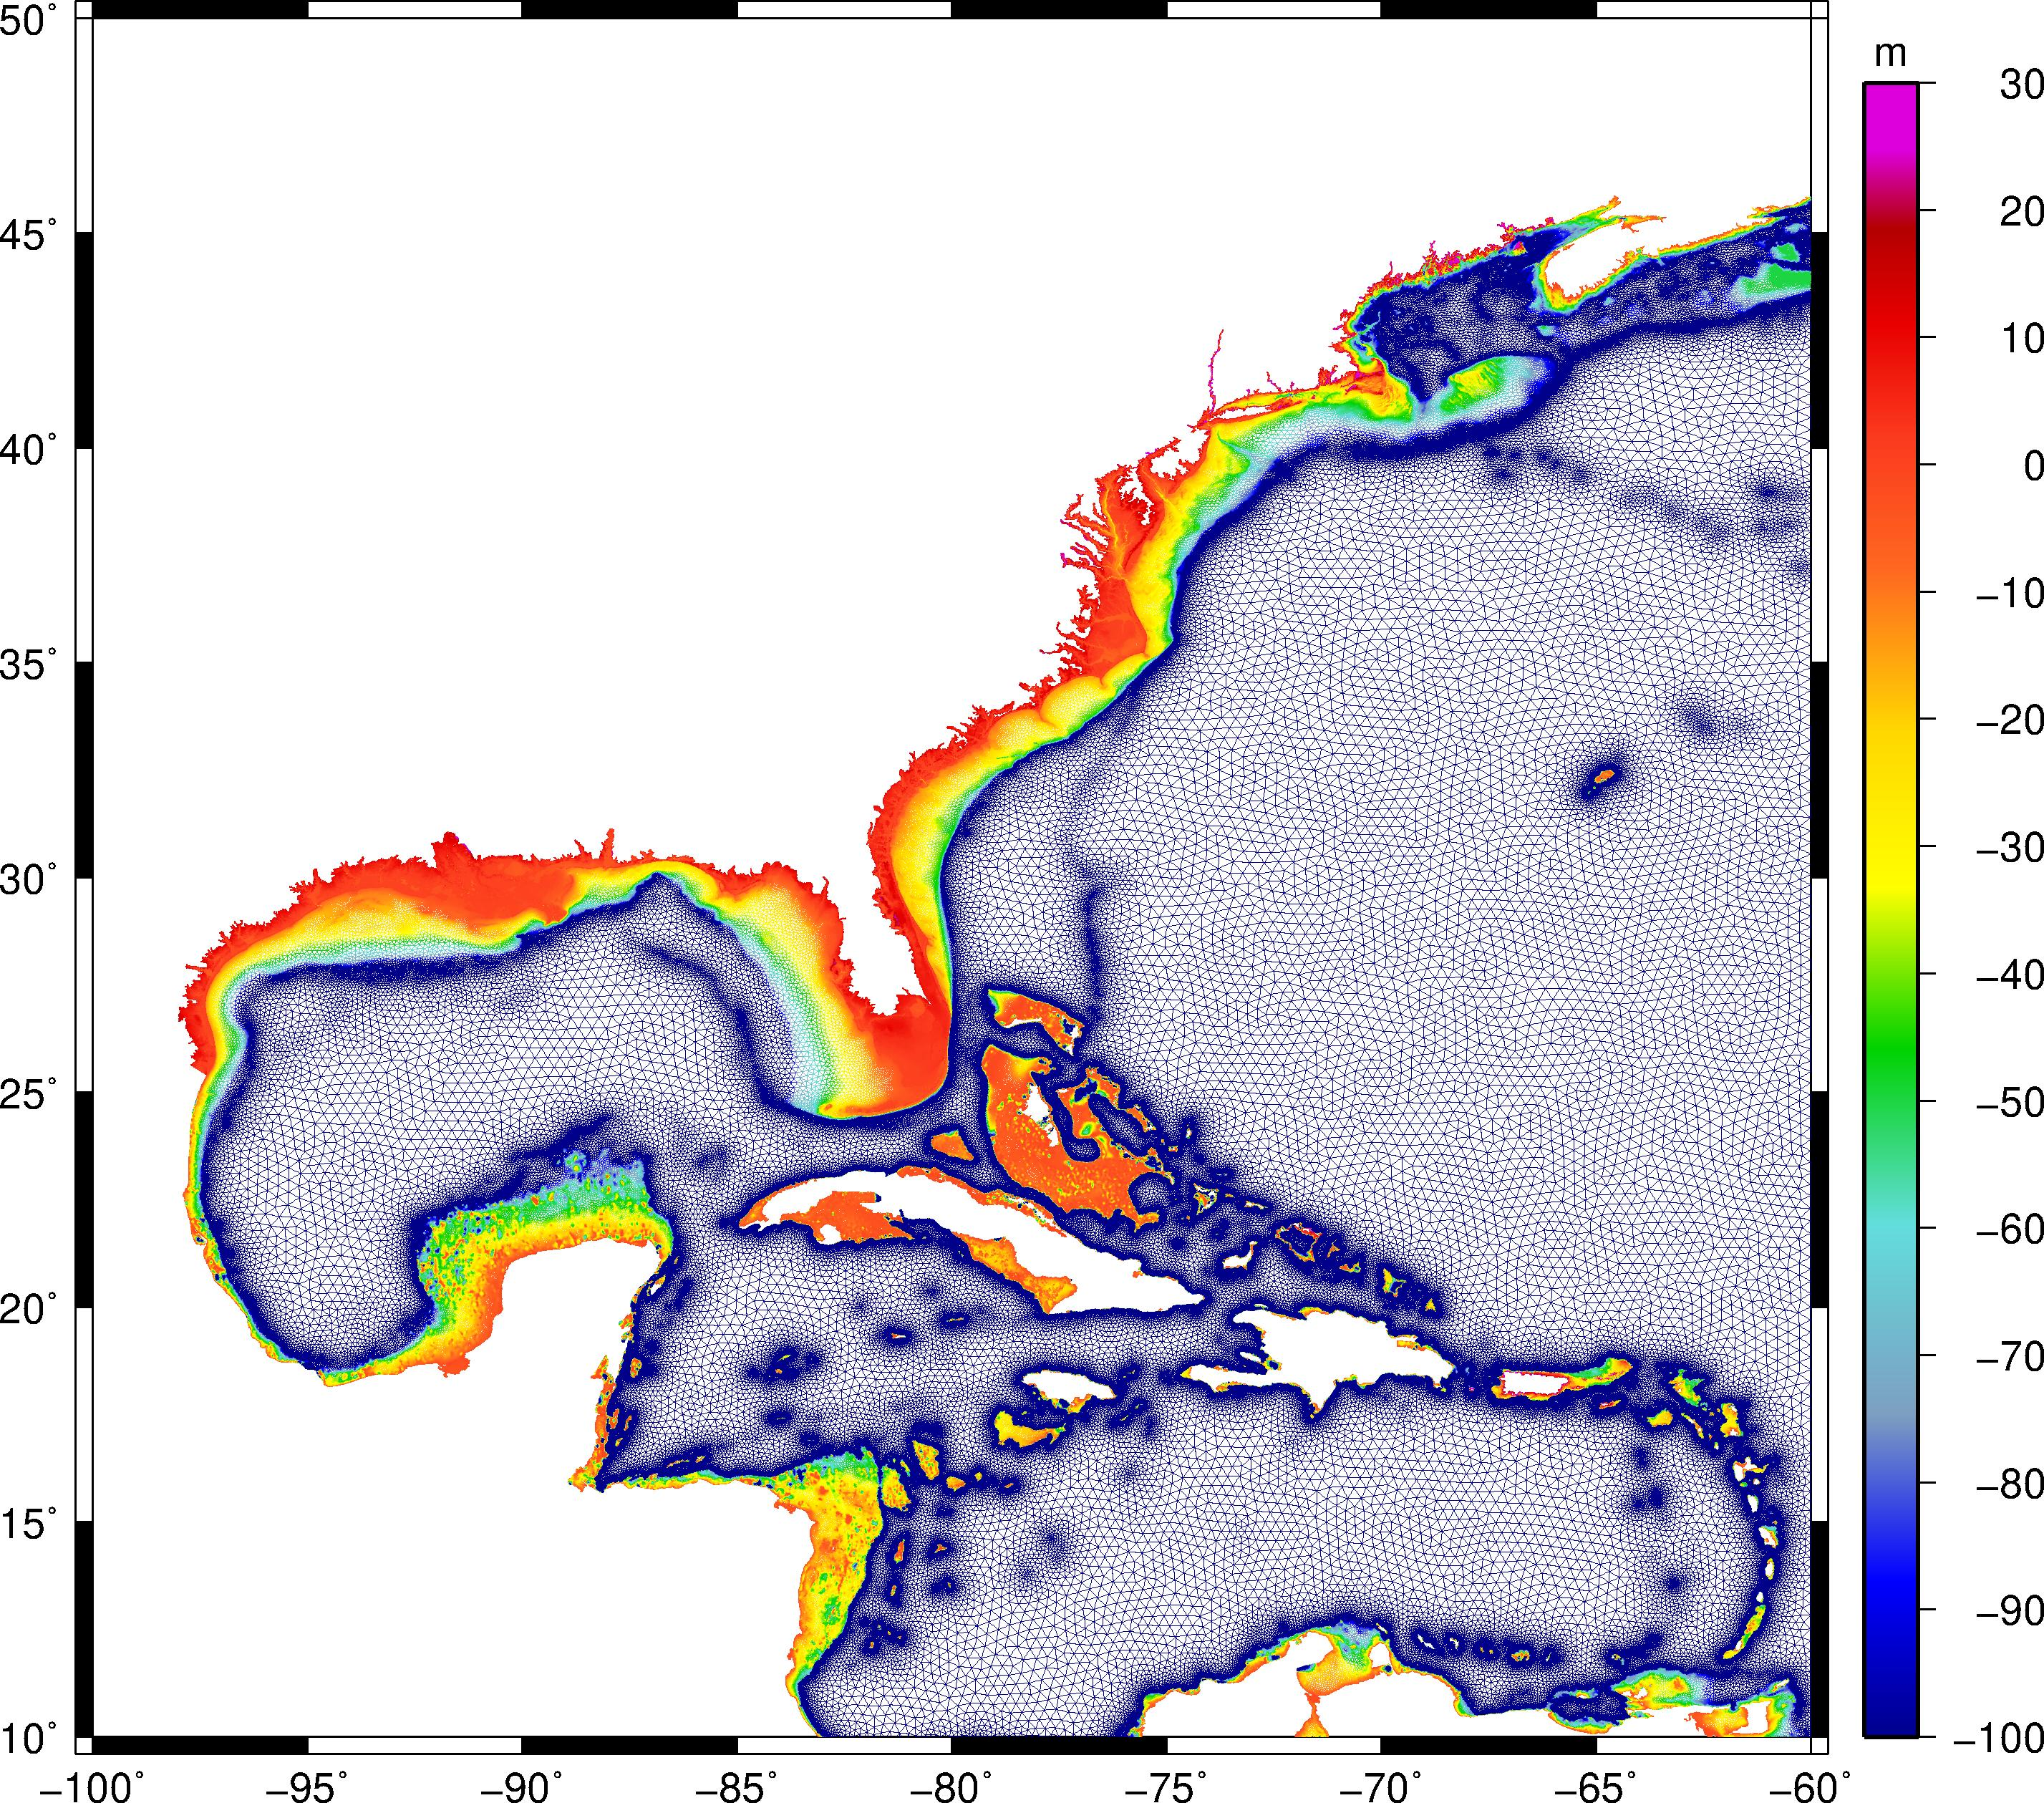
\includegraphics[width=0.75\textwidth]{120m_bath.jpg}
  \end{figure}
\end{frame}

\begin{frame}
  \frametitle{Incorporating rainfall}
  \begin{itemize}
  \item Directly specify rain intensity (m/s) at each node in the grid
    \begin{itemize}
    \item Can be used in hindcasting, given observed rain data
    \item Need to preprocess different types rain data
    \end{itemize}
  \item Use parametric rainfall models
    \begin{itemize}
    \item Rain intensity at each point can be estimated using storm data
    \item If works, useful for forecasting
    \item Comparison of existing parametric models in \\
      \vspace{0.1cm}
      \ul{Brackins and Kalyanapu (2019). \emph{Evaluation of Parametric Precipitation Models in Reproducing Tropical Cyclone Rainfall Patterns}. Journal of Hydrology.}
    \end{itemize}
  \end{itemize}
\end{frame}
\begin{frame}
  \frametitle{R-CLIPER Rain Model}
  \begin{itemize}
  \item Based on the work of Lonfat et al. (2004) and Marks and DeMaria (2003)
  \item Curve fitting using Tropical Rainfall Measurement Mission (TRMM)  rainfall data from storm between 1998-2002:
    \begin{align}
      TRR(r, V) =
    \begin{cases}
      T_0 + (T_m - T_0)(r/r_m), & r < r_m \\
      T_m e^{-((r-rm)/r_e)}, & r \geq r_m
    \end{cases}
    \end{align}
    where
    \begin{align*}
      TRR &= \text{rain rate (inch/day) at a given point} \\
      r &= \text{radius from the point to the center of the storm} \\
      V &= \text{maximum wind speed}
    \end{align*}
  \end{itemize}
\end{frame}

\begin{frame}
  \frametitle{Storm data}
  \begin{itemize}
  \item ADCIRC and DG-SWEM accepts wind and atmospheric pressure input in Best Track format
  \end{itemize}
\end{frame}

\begin{frame}
  \frametitle{Test case: Hurricane Harvey (2017)}
  \begin{columns}
    \column{0.5\linewidth}
  \begin{itemize}
  \item Maximum total rain of 51 inches in the Houston city area
  \item Surge relatively low
  \item Simulation dates: August 23 - September 2, 2017
  \item Used 3,200 processors, took about 13 hours on the Texas Advanced Computing Center (TACC)
  \end{itemize}

  \column{0.5\linewidth}
  \centering
  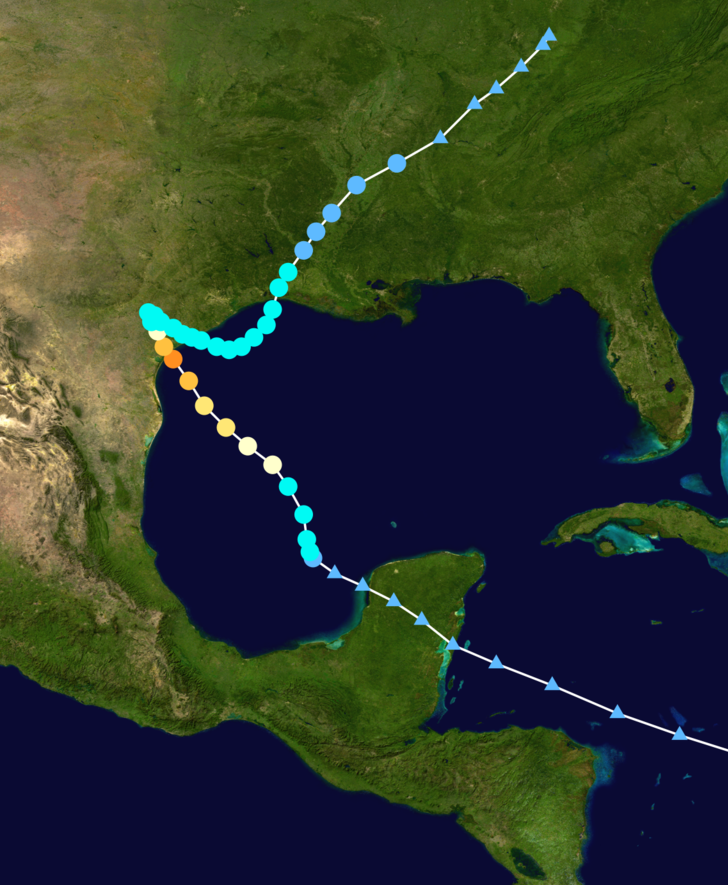
\includegraphics[width=0.8\linewidth]{harvey_cropped.png} \\
  \footnotesize Track of Hurricane Harvey (2017)
  \end{columns}

\end{frame}


\begin{frame}
  \frametitle{Hydrograph locations}
  \centering
  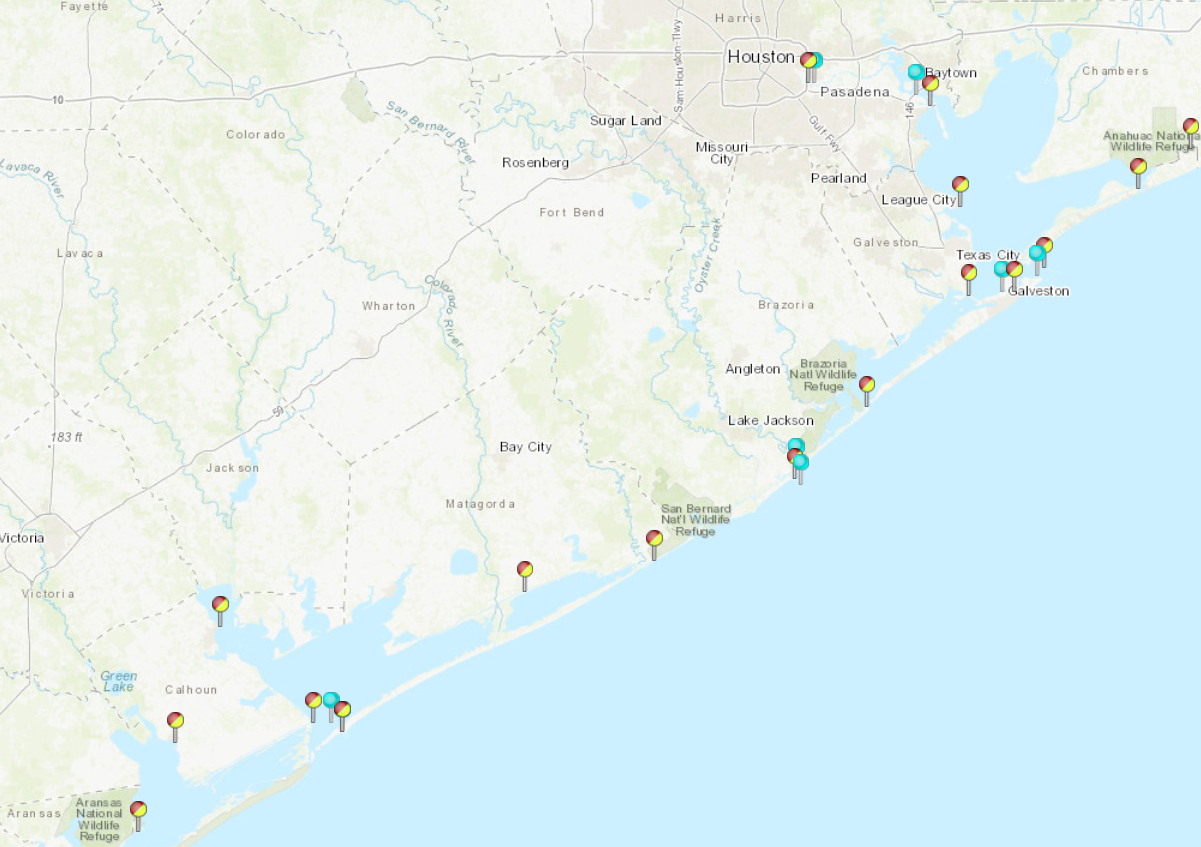
\includegraphics[width=0.9\linewidth]{stations.png}
\end{frame}


\begin{frame}
  \frametitle{Results - Hydrograph Comparisons}
  \centering
  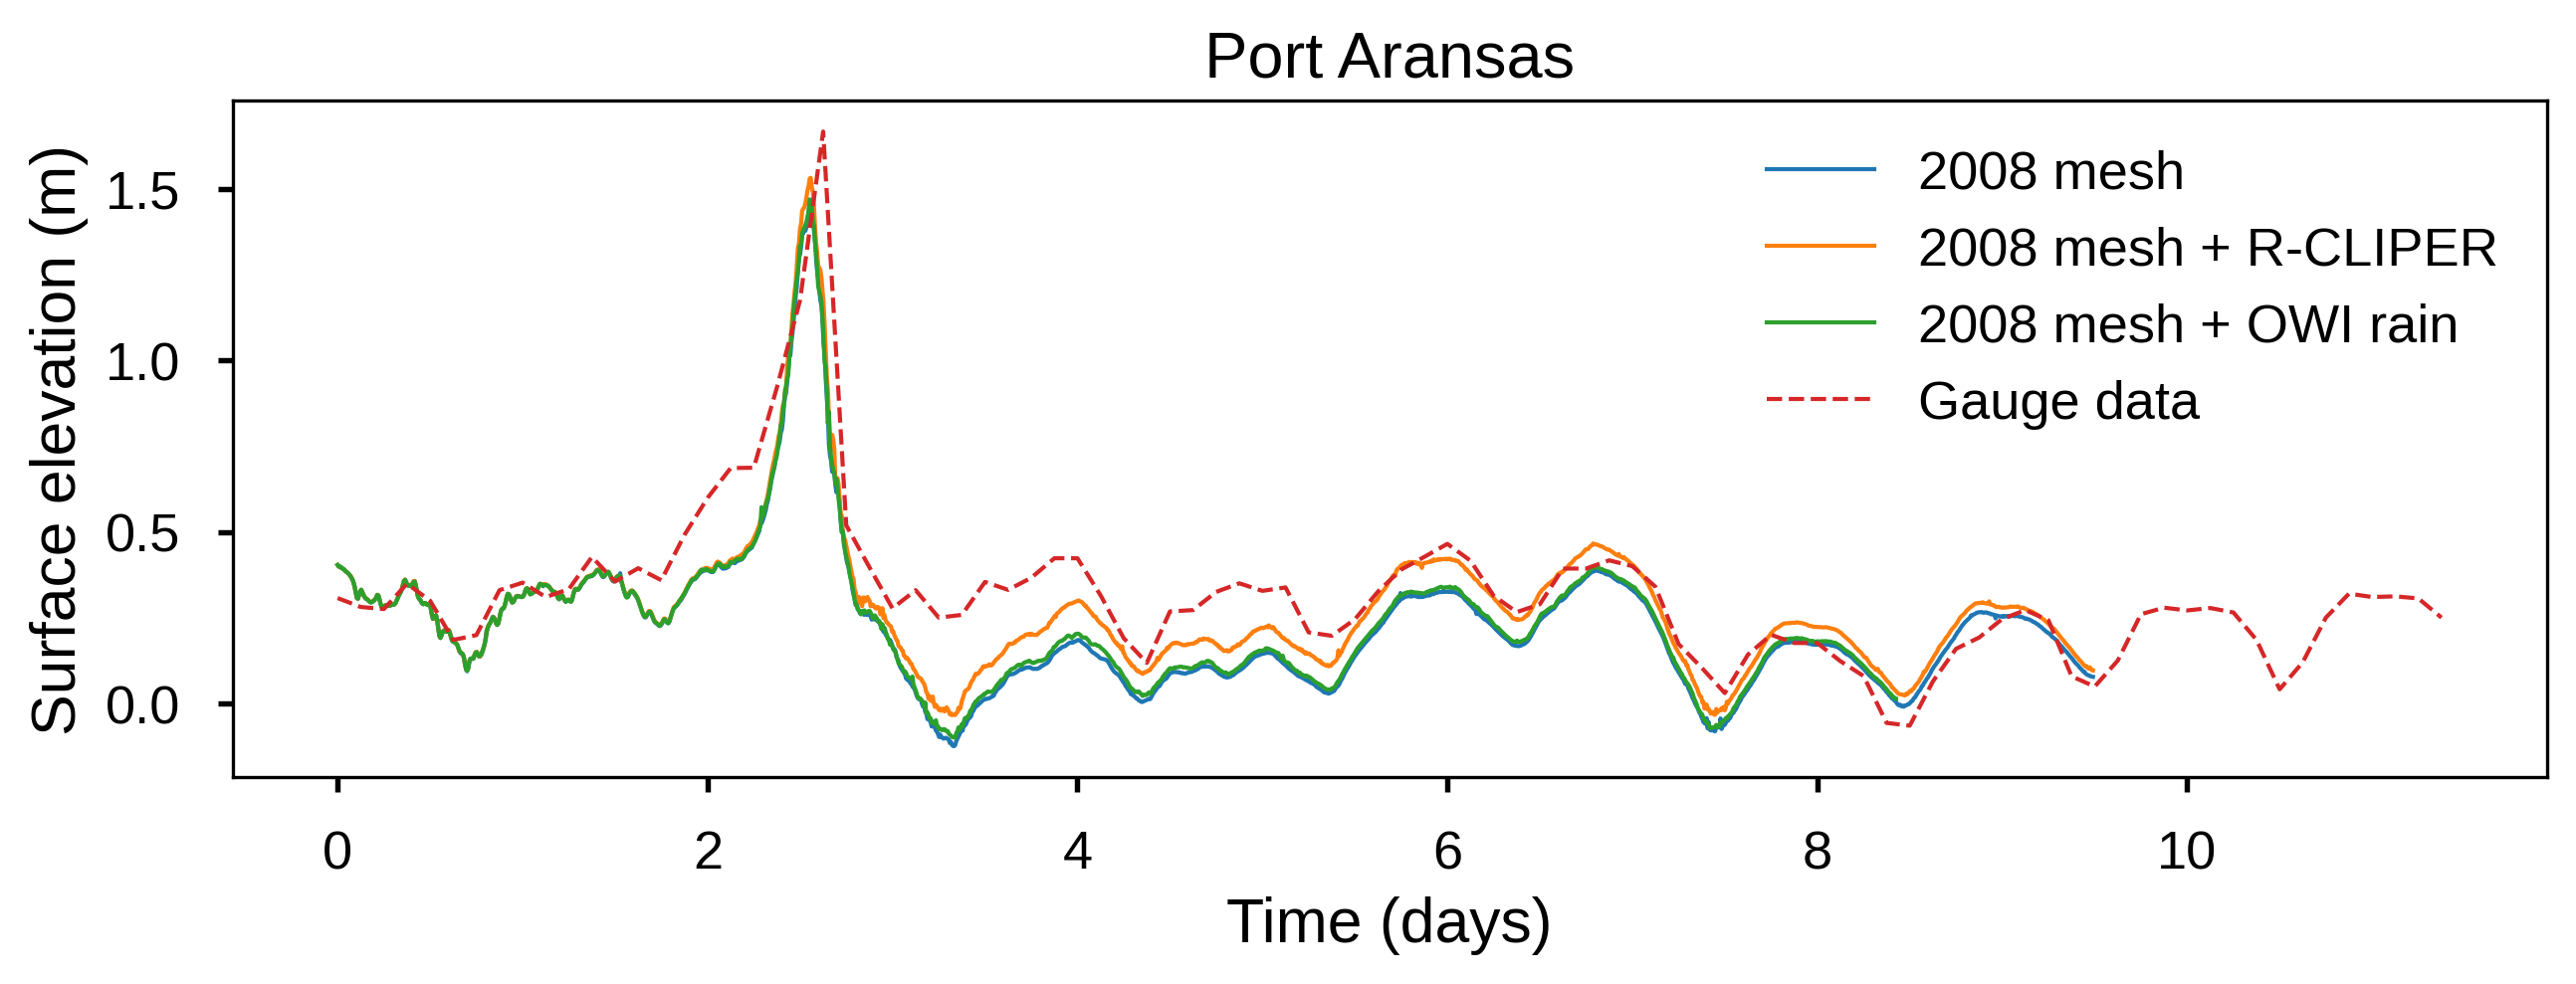
\includegraphics[width=0.9\linewidth]{port_aransas.png}
  \centering
  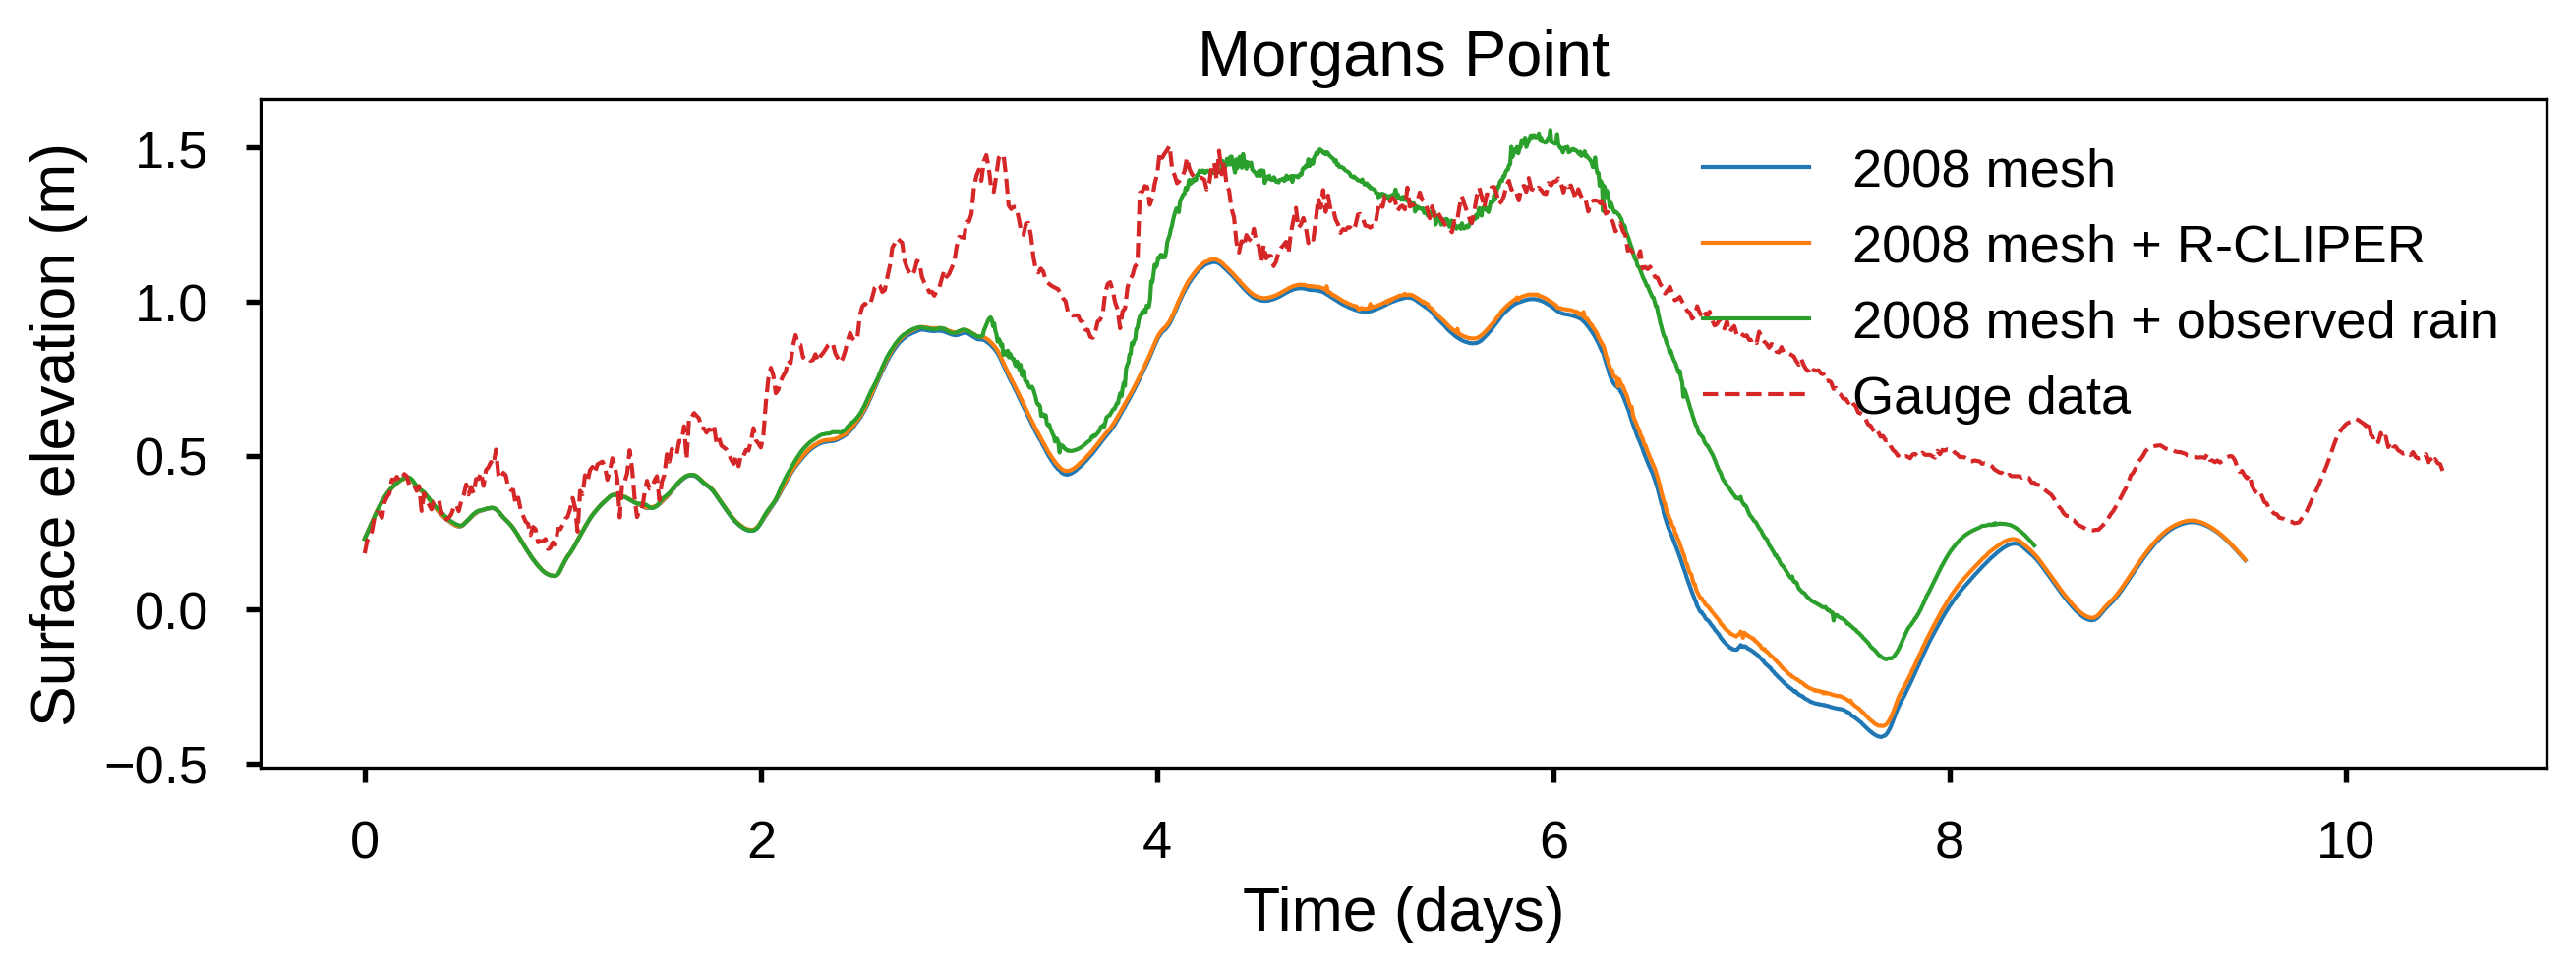
\includegraphics[width=0.9\linewidth]{morgans_point.png}
\end{frame}

\begin{frame}
  \frametitle{Results - Hydrograph Comparisons}
  \centering
  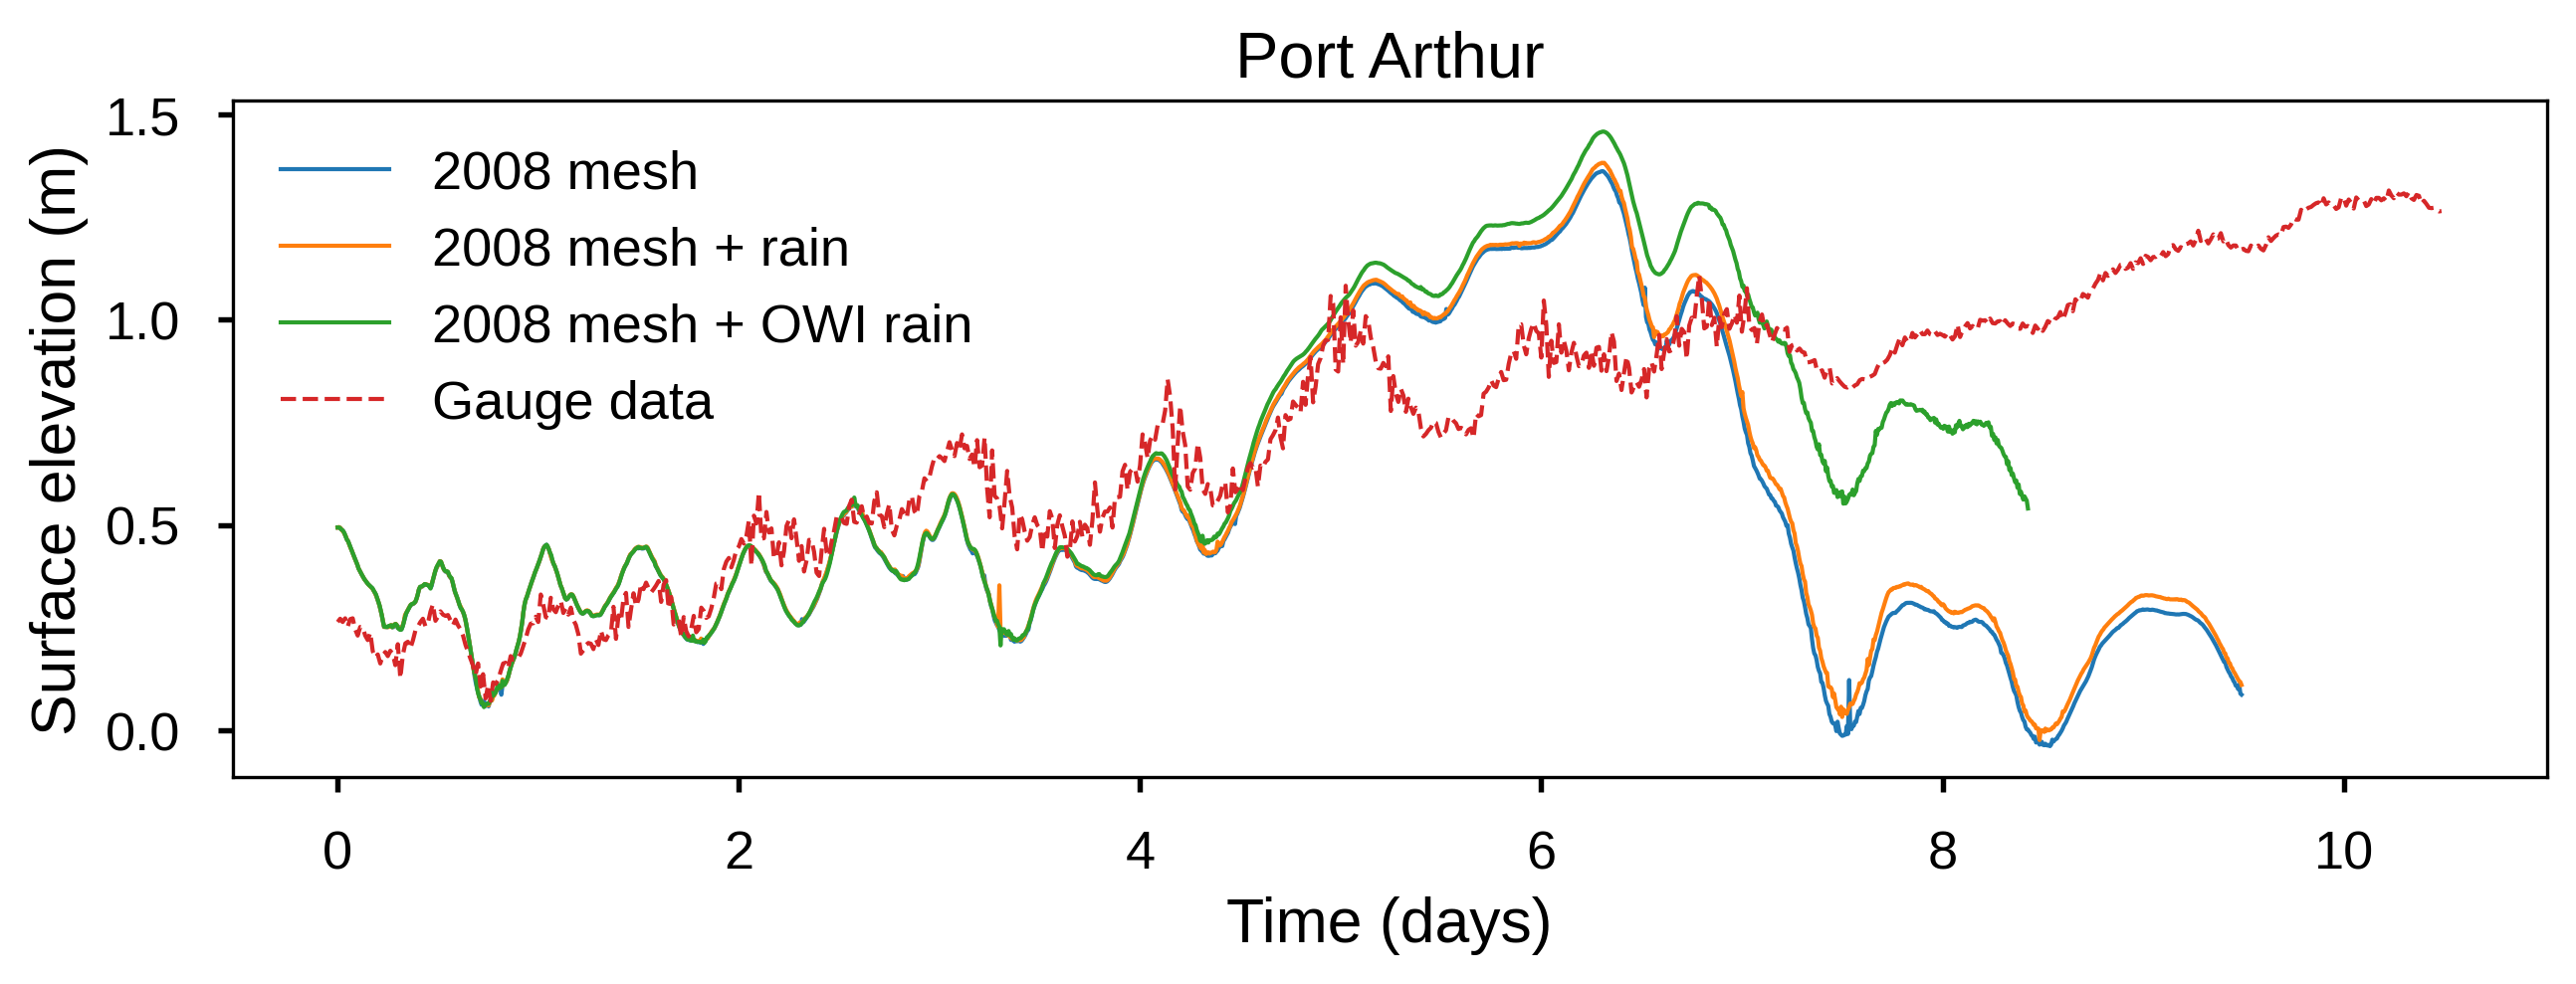
\includegraphics[width=0.9\linewidth]{port_arthur.png}
  \centering
  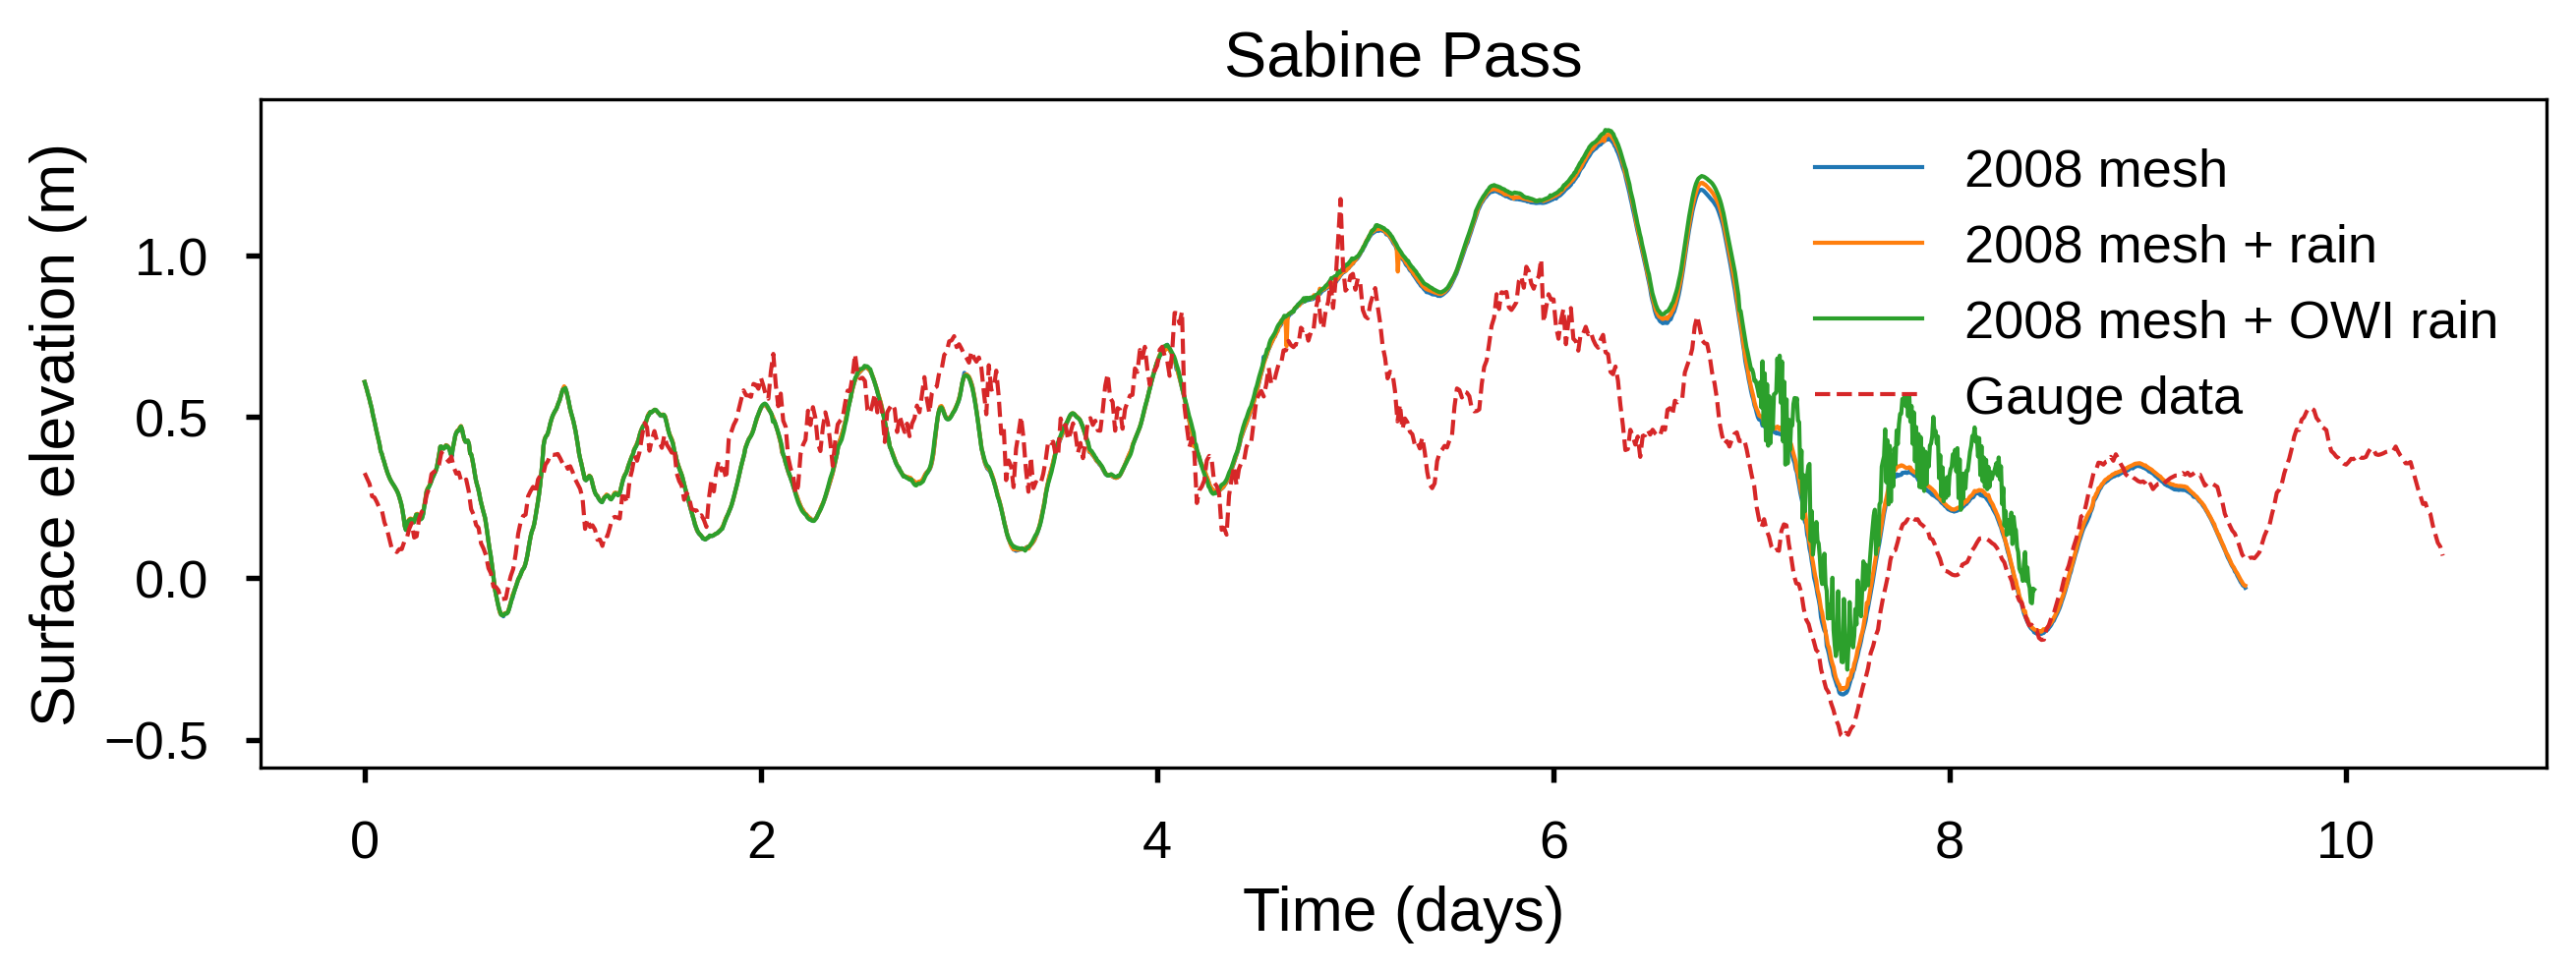
\includegraphics[width=0.9\linewidth]{sabine_pass.png}
\end{frame}

\begin{frame}
  \frametitle{Results - Hydrograph Comparisons}
  \centering
  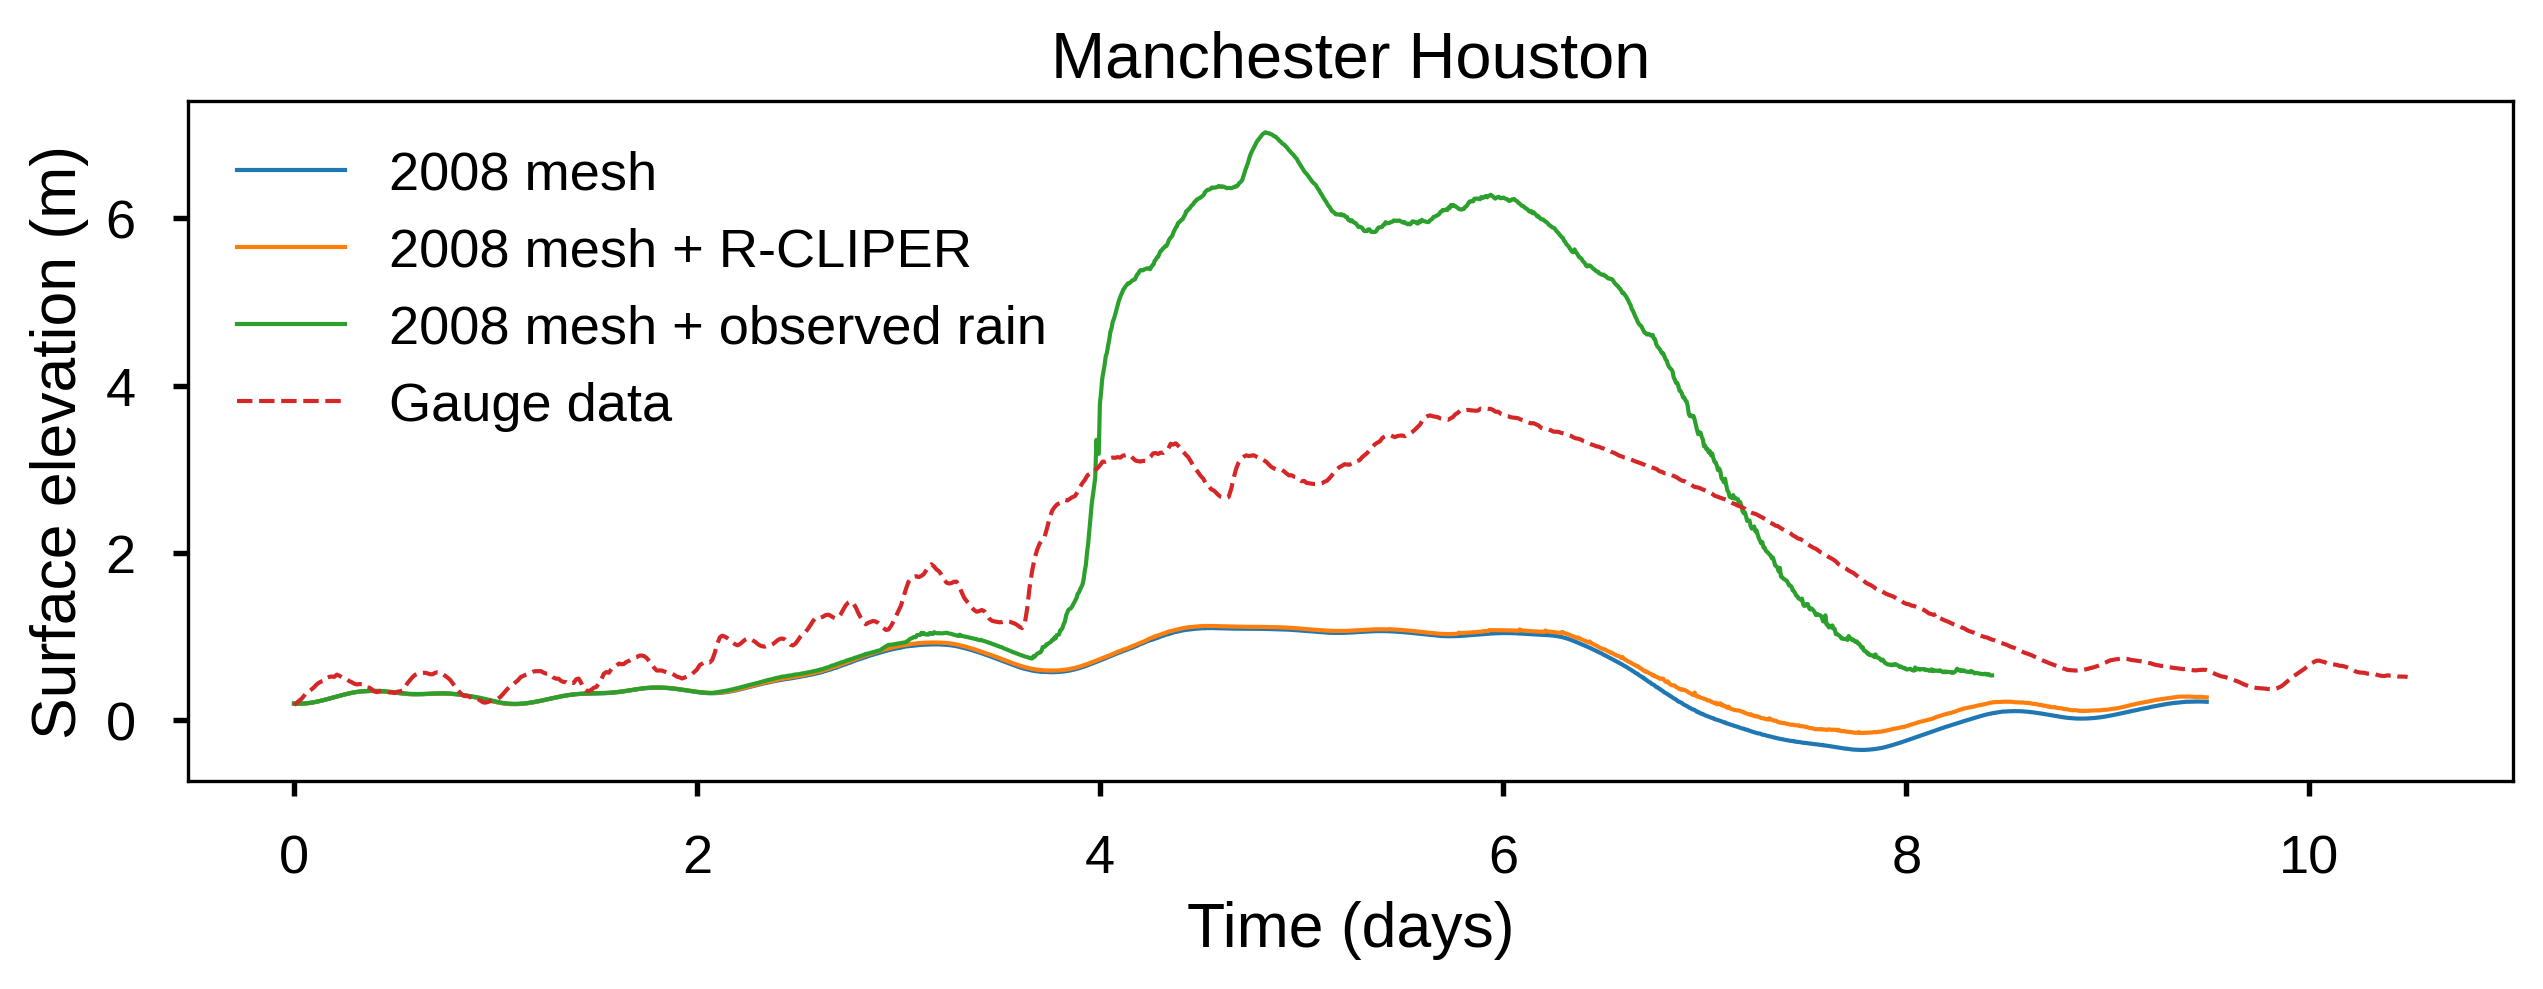
\includegraphics[width=0.9\linewidth]{manchester.png}
  \centering
  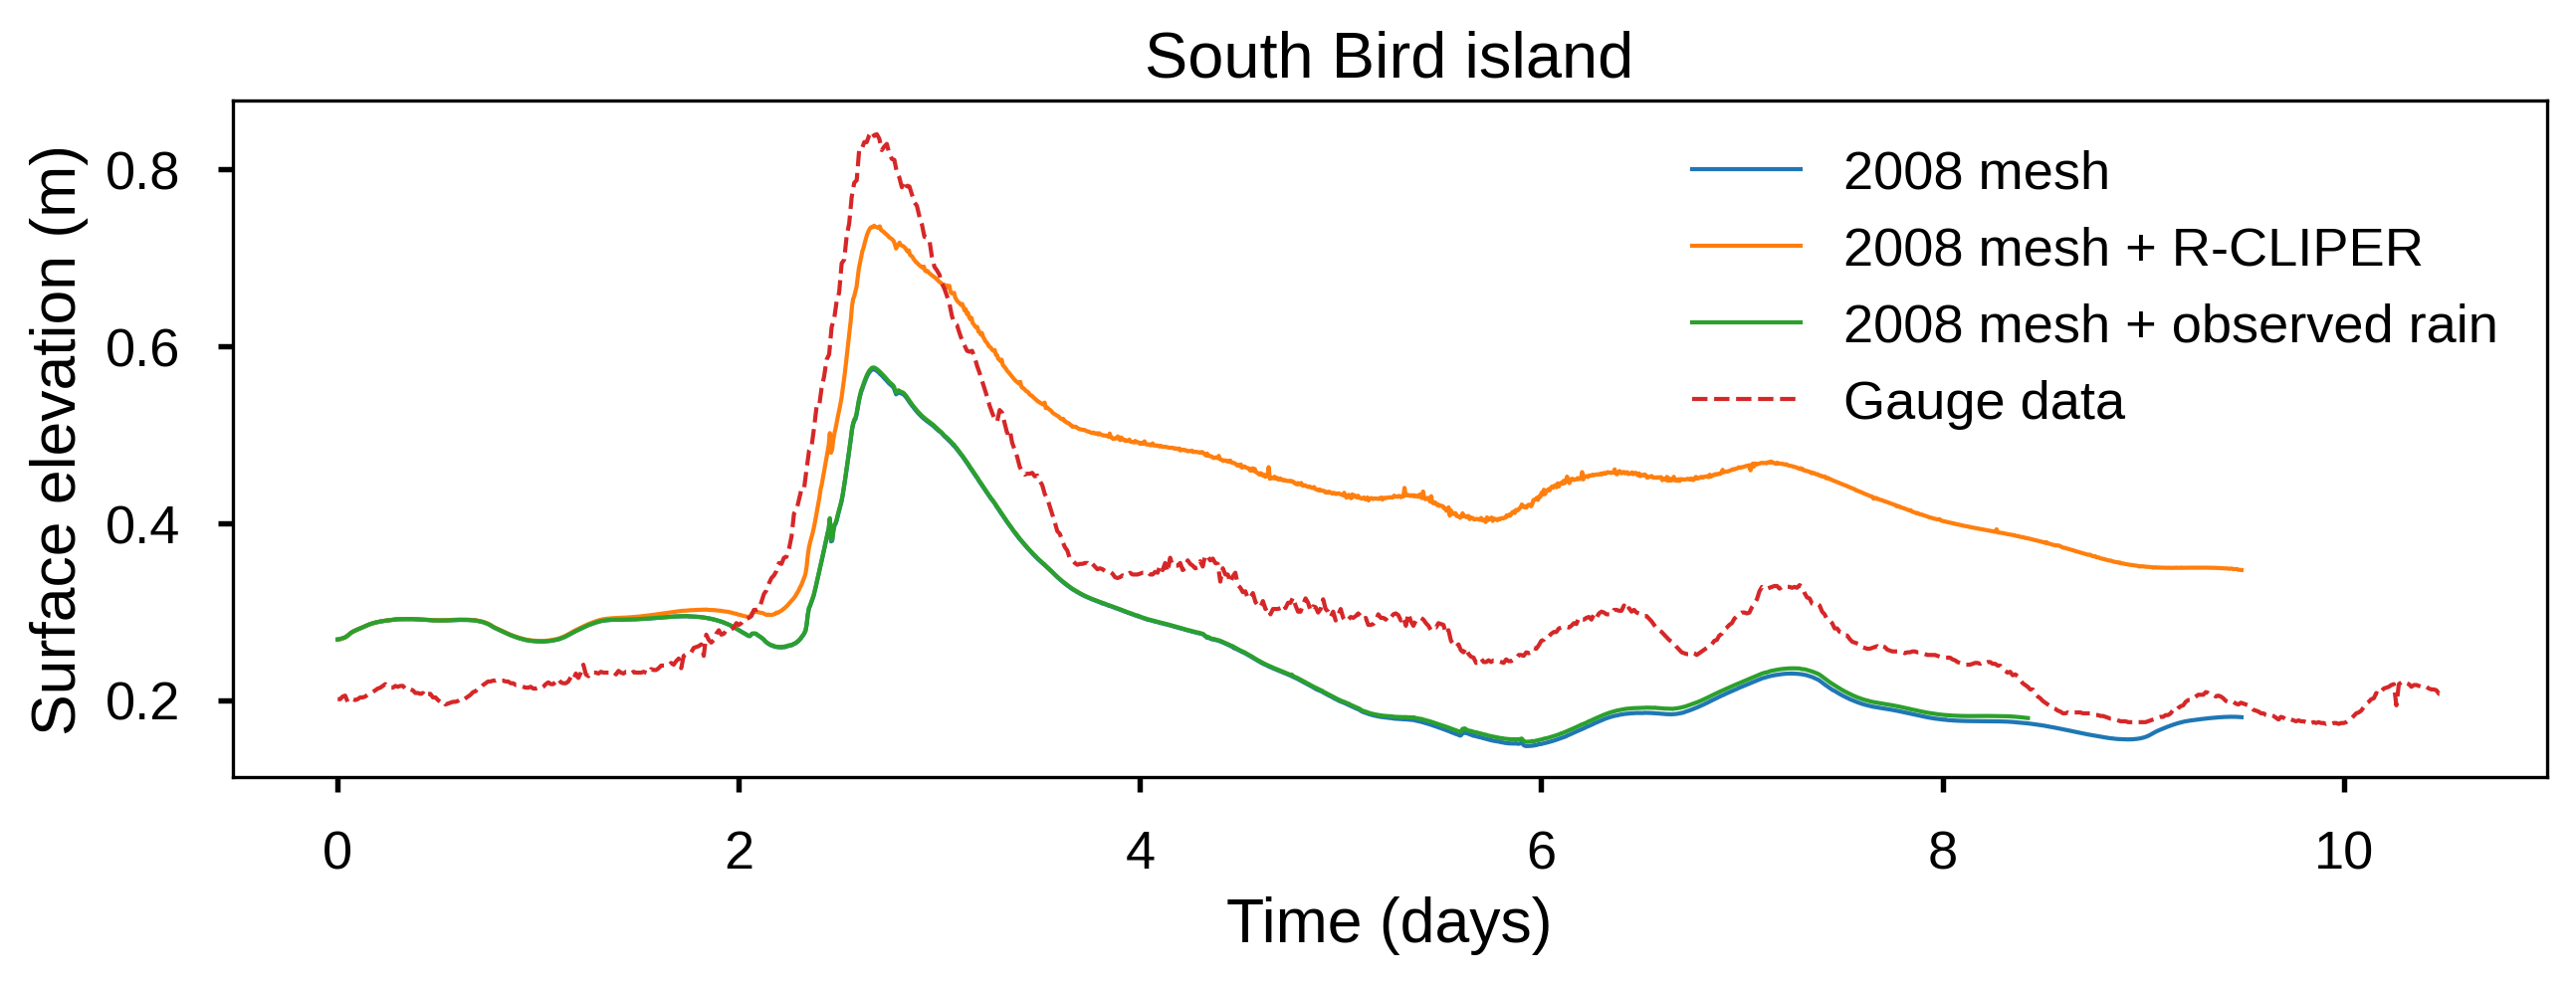
\includegraphics[width=0.9\linewidth]{south_bird.png}
\end{frame}

\begin{frame}
  \frametitle{Results - Hydrograph Comparisons}
  \centering
  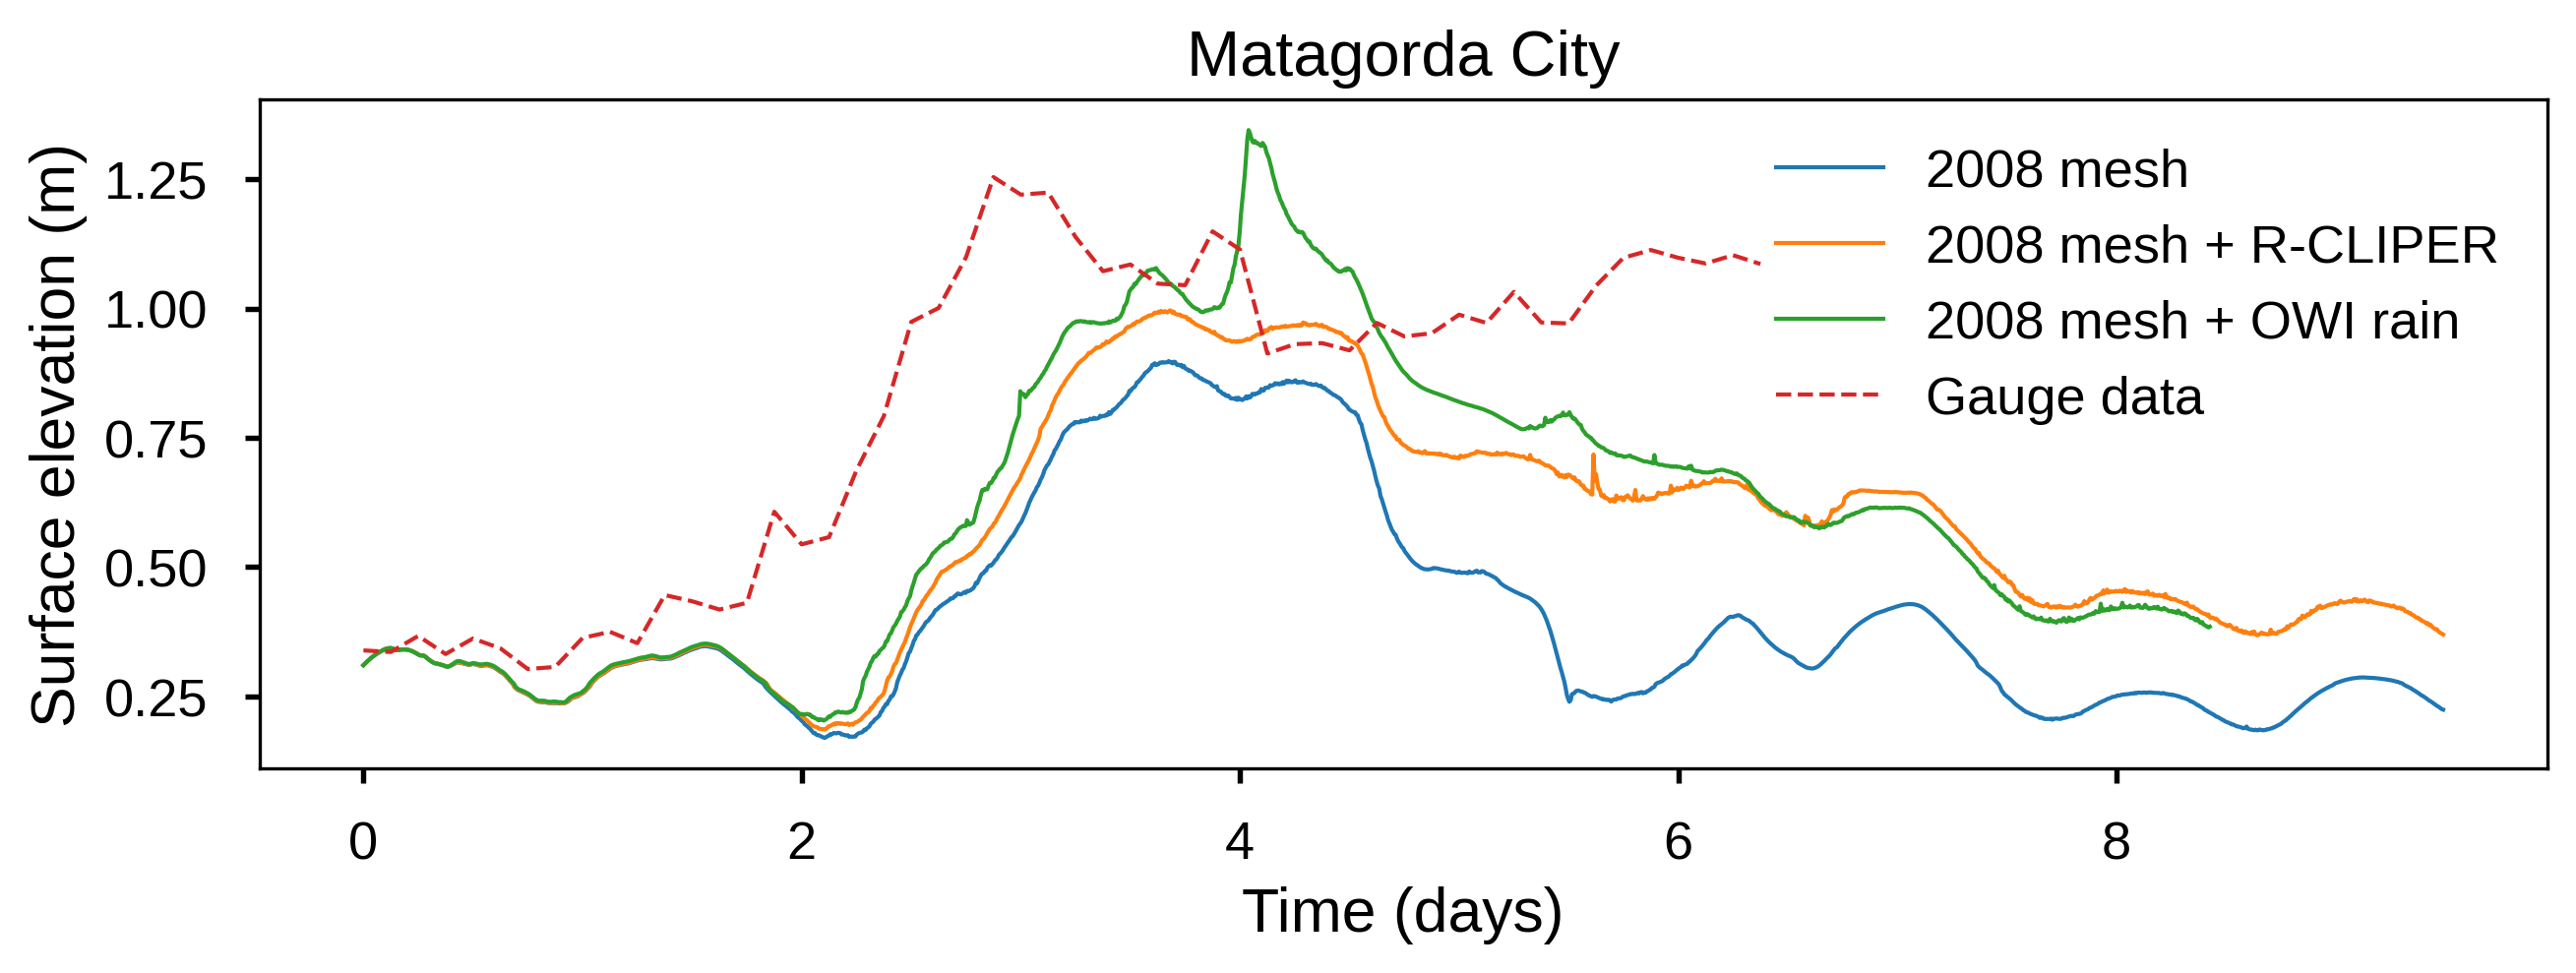
\includegraphics[width=0.9\linewidth]{matagorda.png}
  \centering
  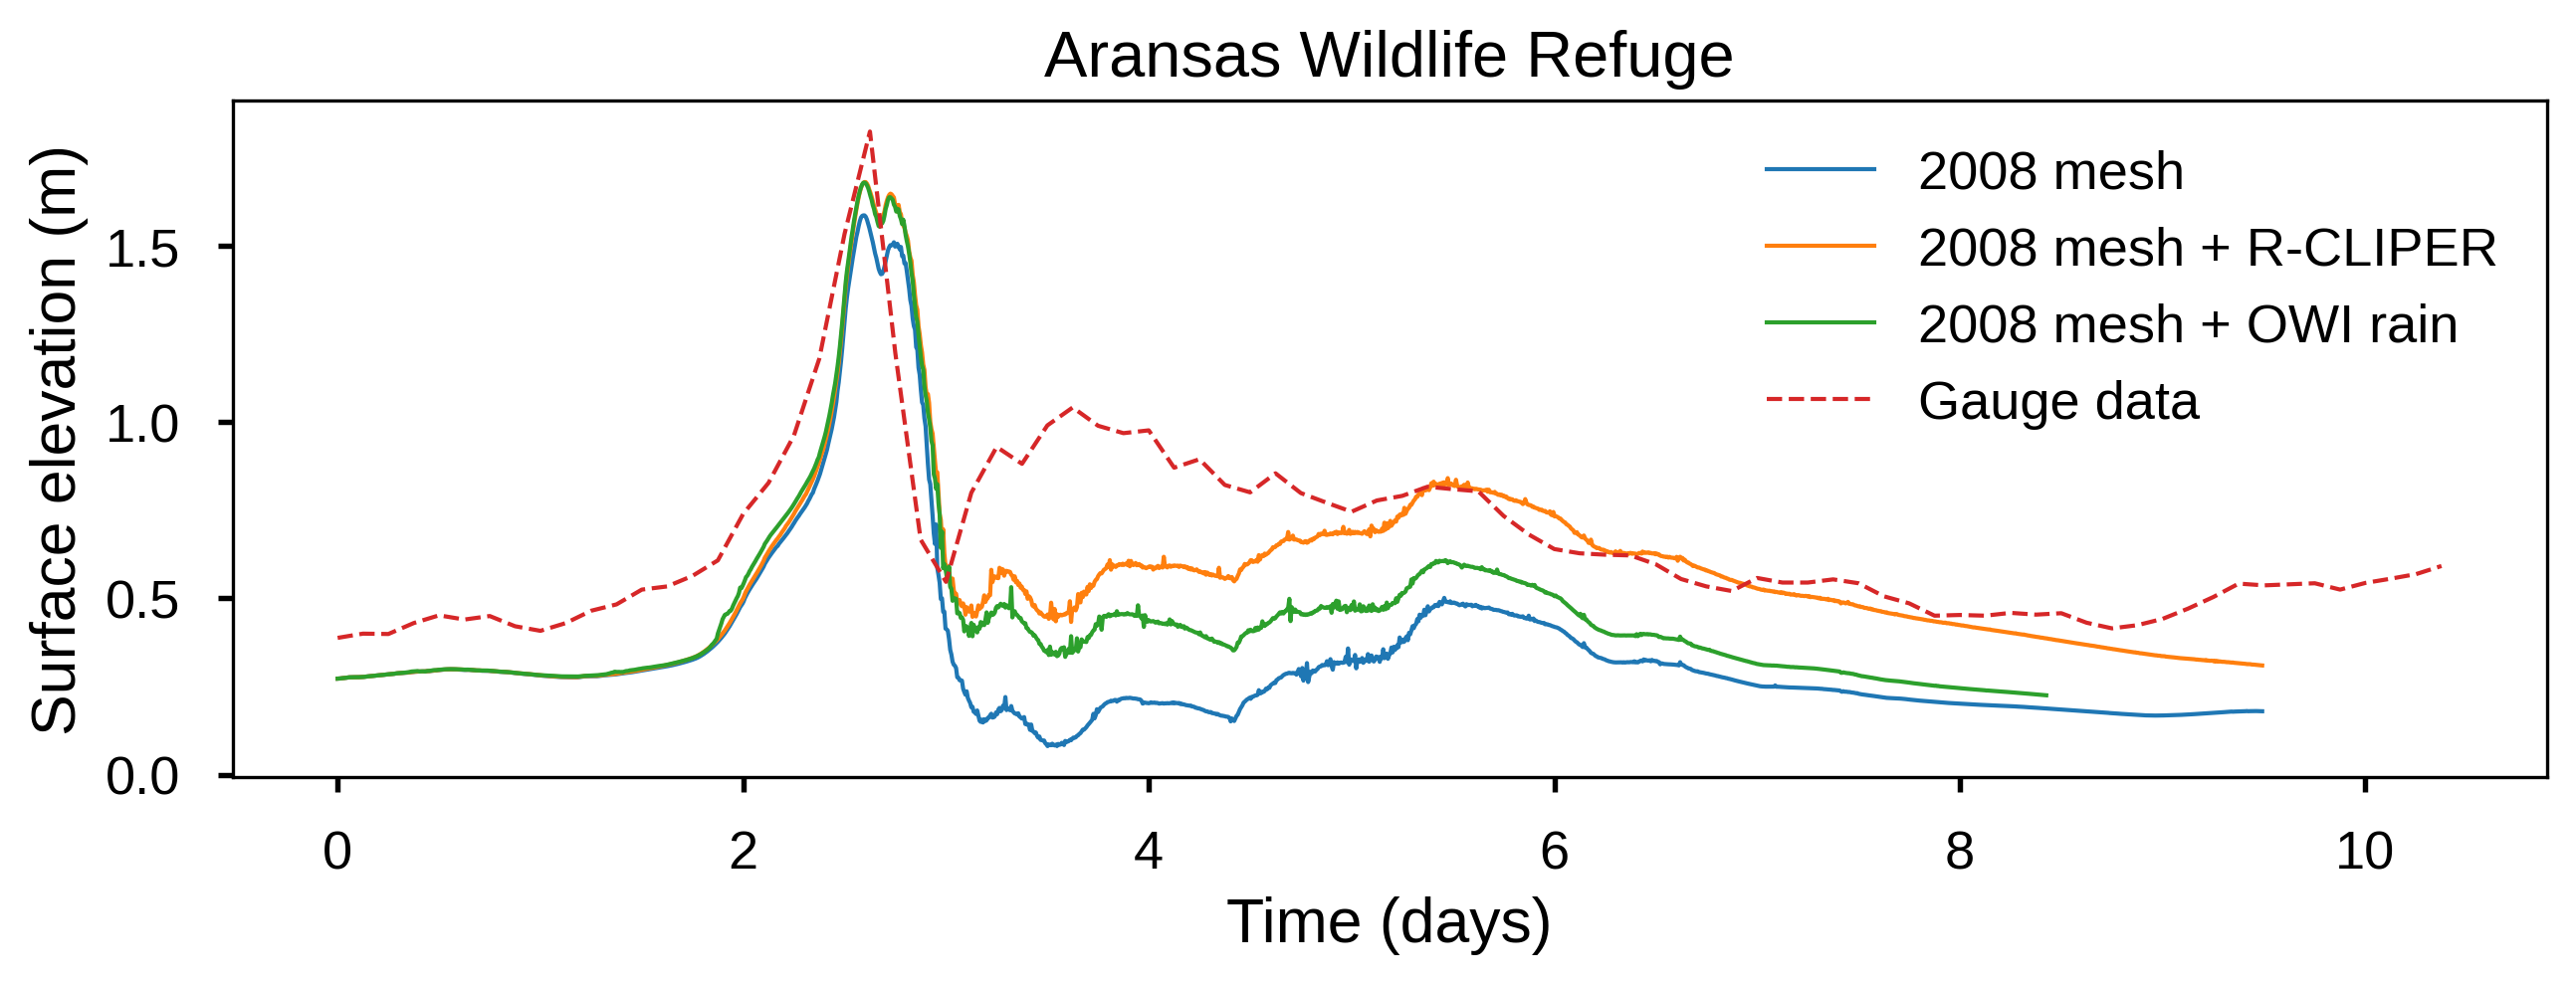
\includegraphics[width=0.9\linewidth]{aransas_wildlife.png}
\end{frame}

\begin{frame}
  \frametitle{Results - Hydrograph Comparisons}
  \centering
  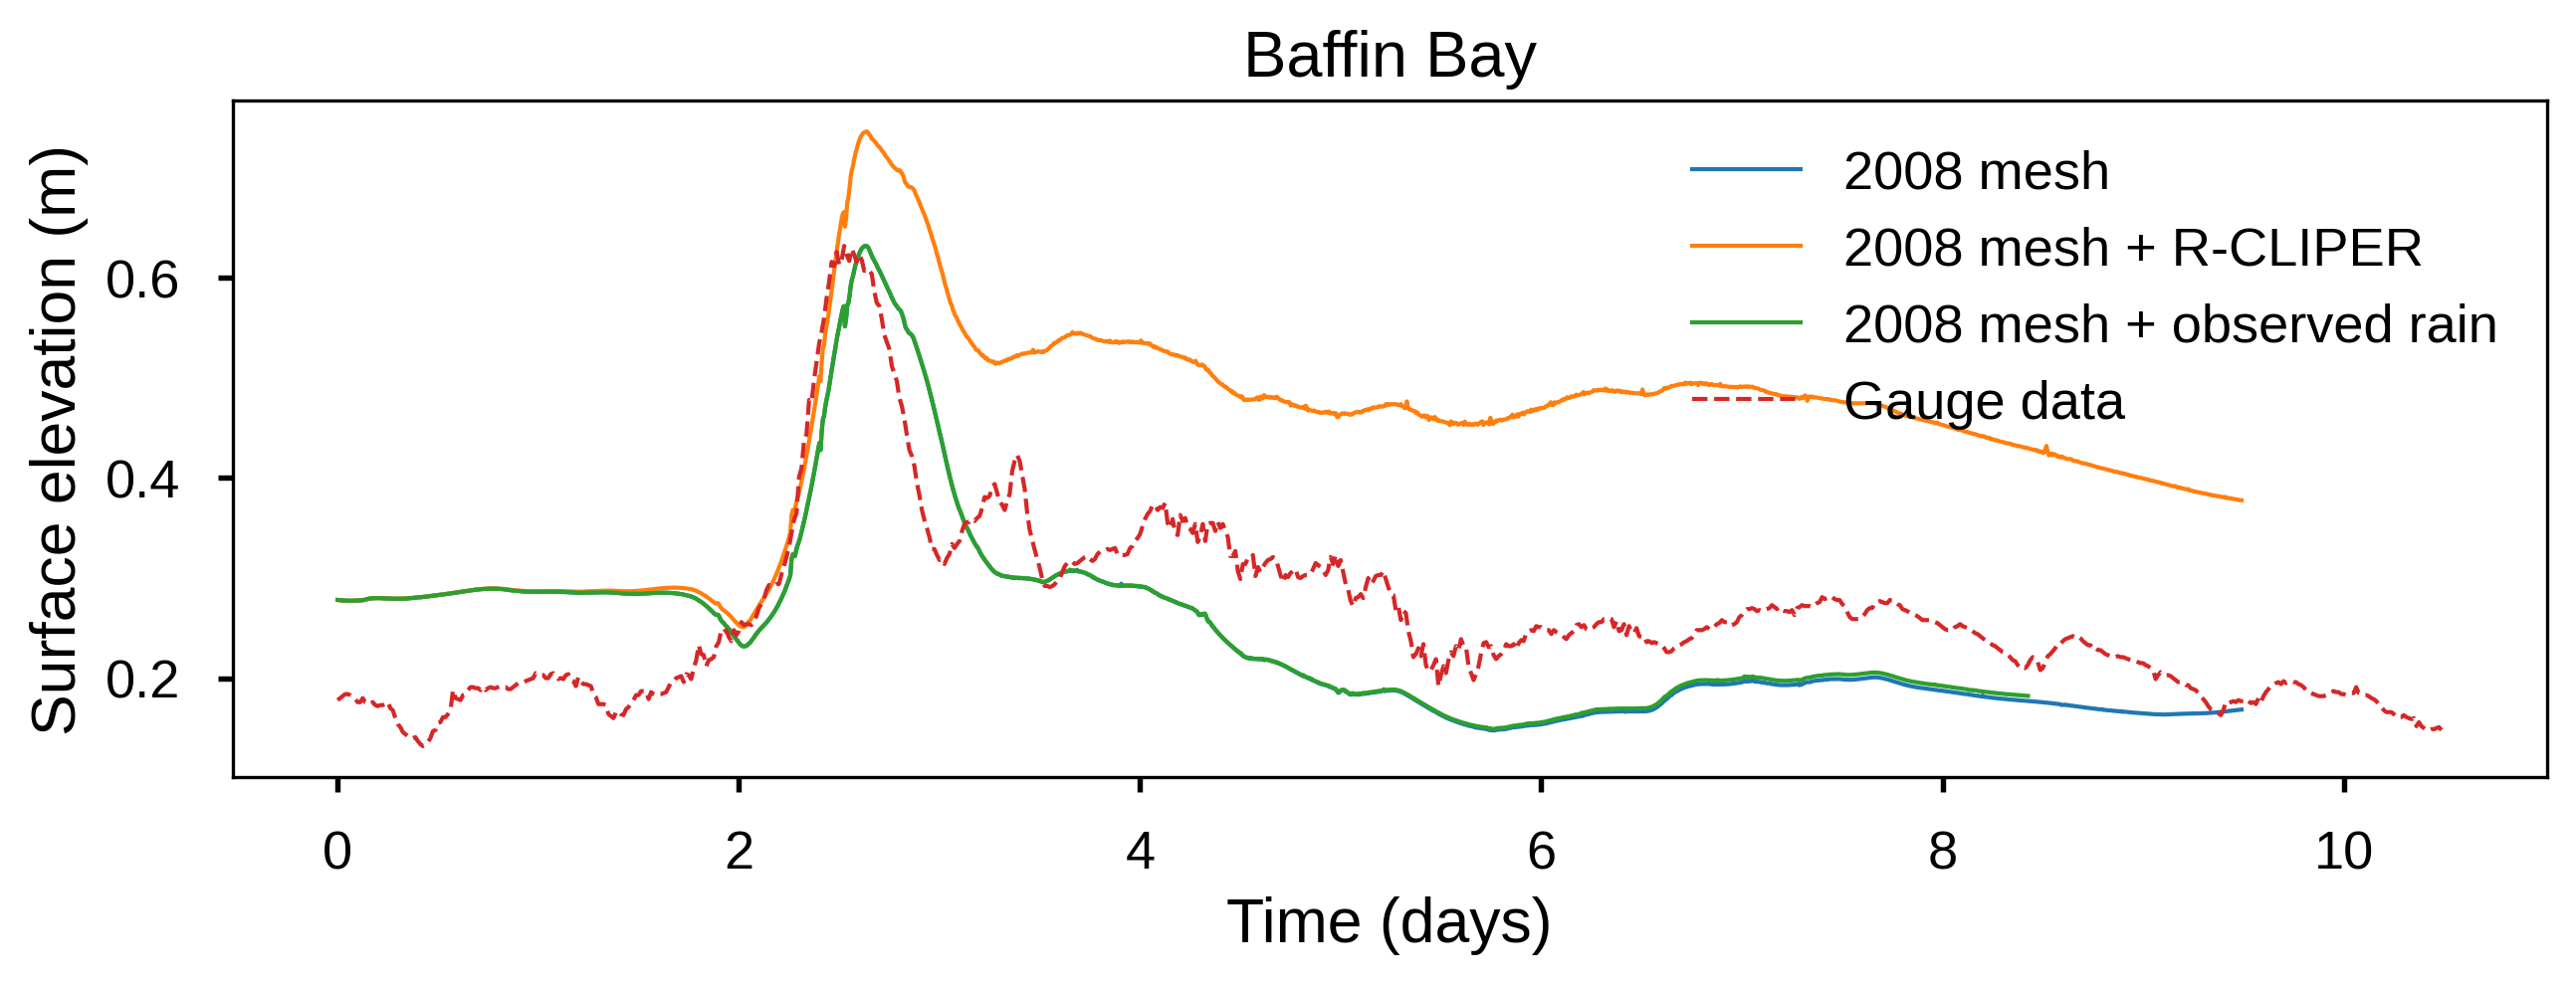
\includegraphics[width=0.9\linewidth]{baffin_bay.png}
  \centering
  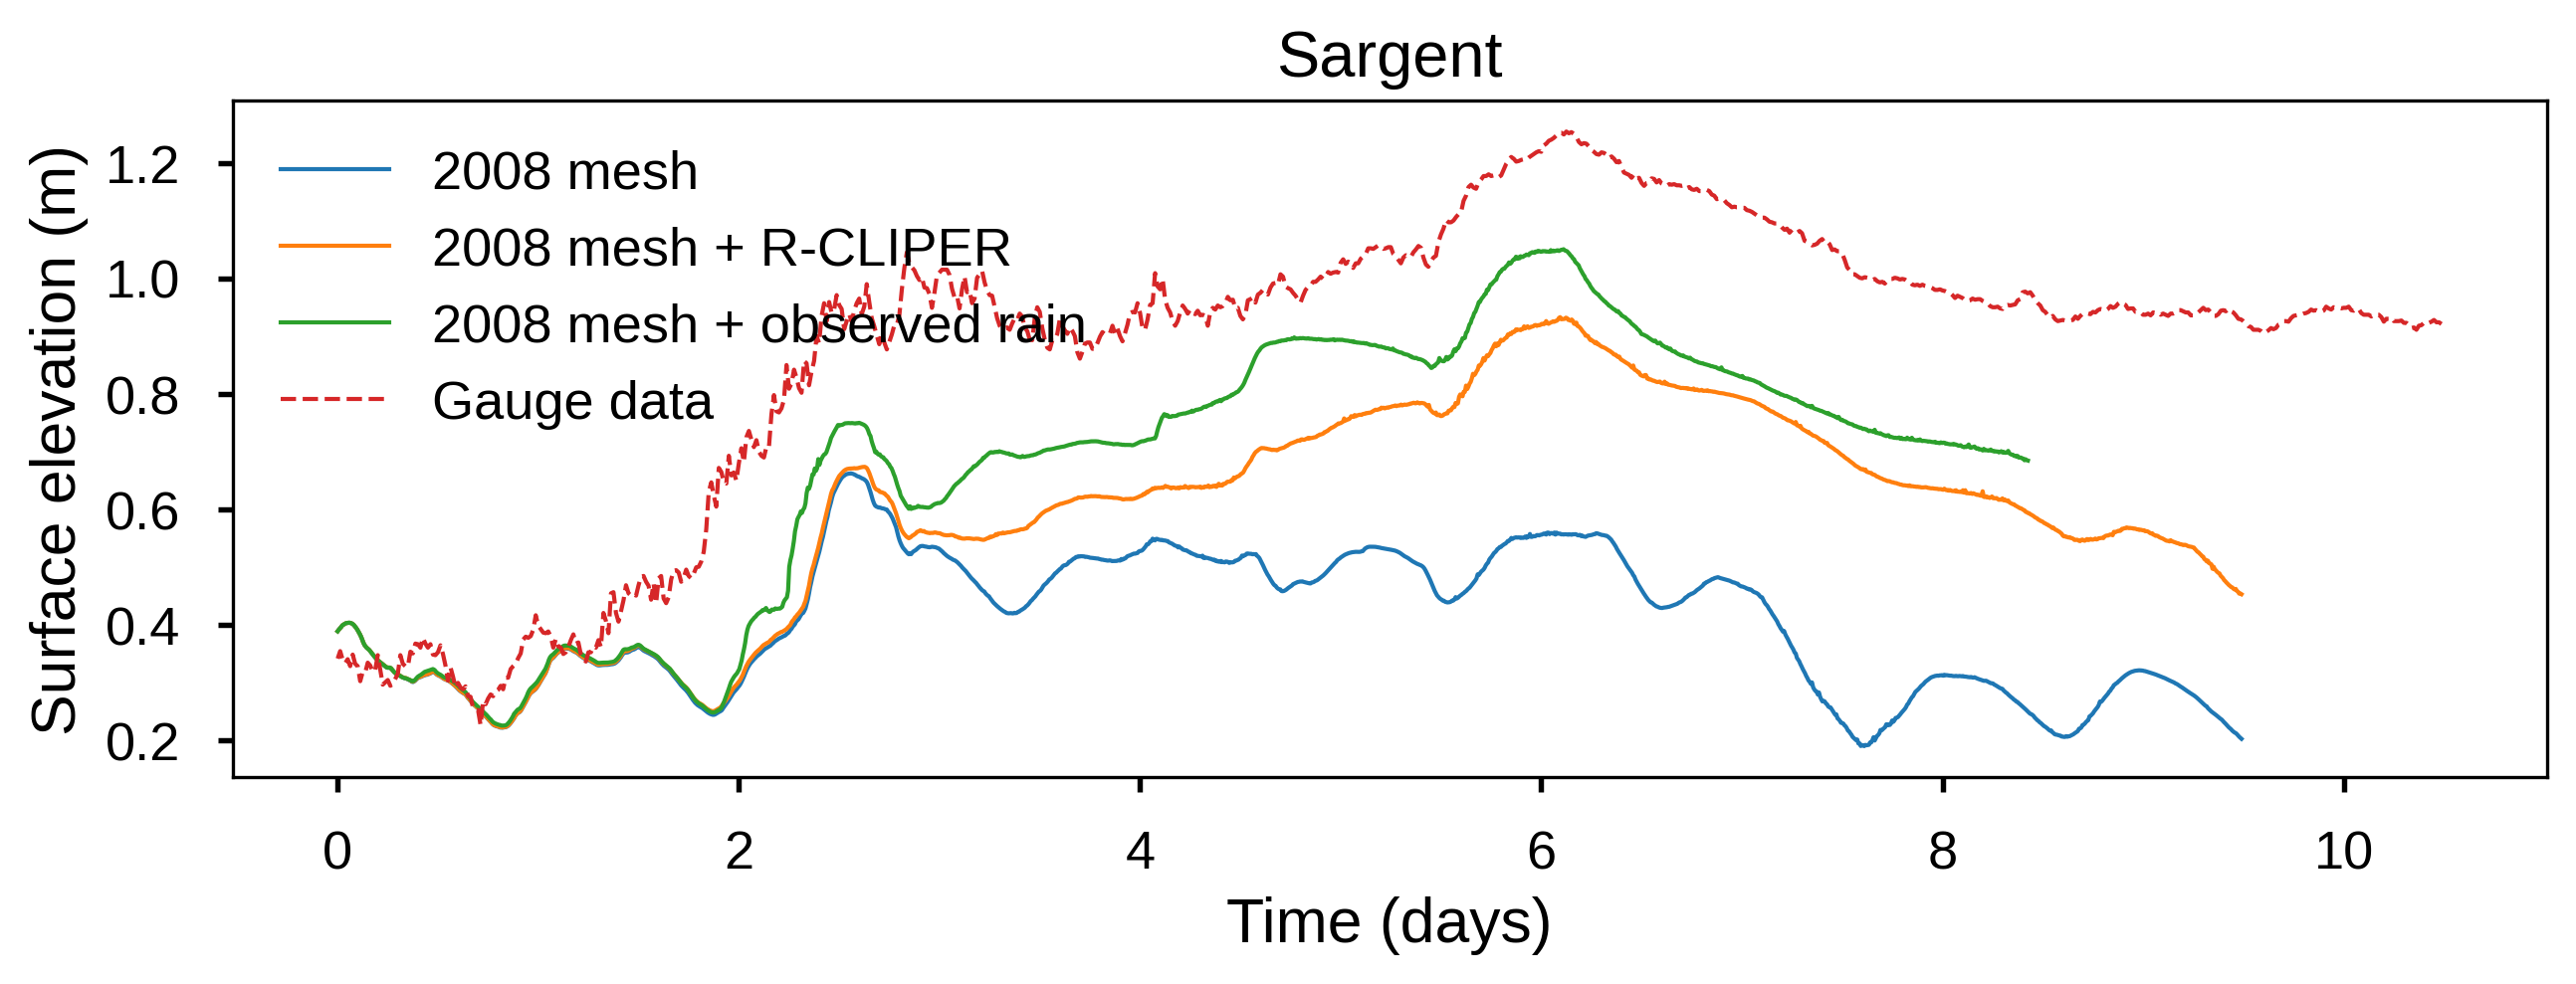
\includegraphics[width=0.9\linewidth]{sargent.png}
\end{frame}

\begin{frame}
  \frametitle{Results - High Water Marks Comparisons}
  \begin{columns}
    \column{0.5\linewidth}
    \centering
    \vspace{0.5cm}
    \centering
    DG-SWEM without rainfall
    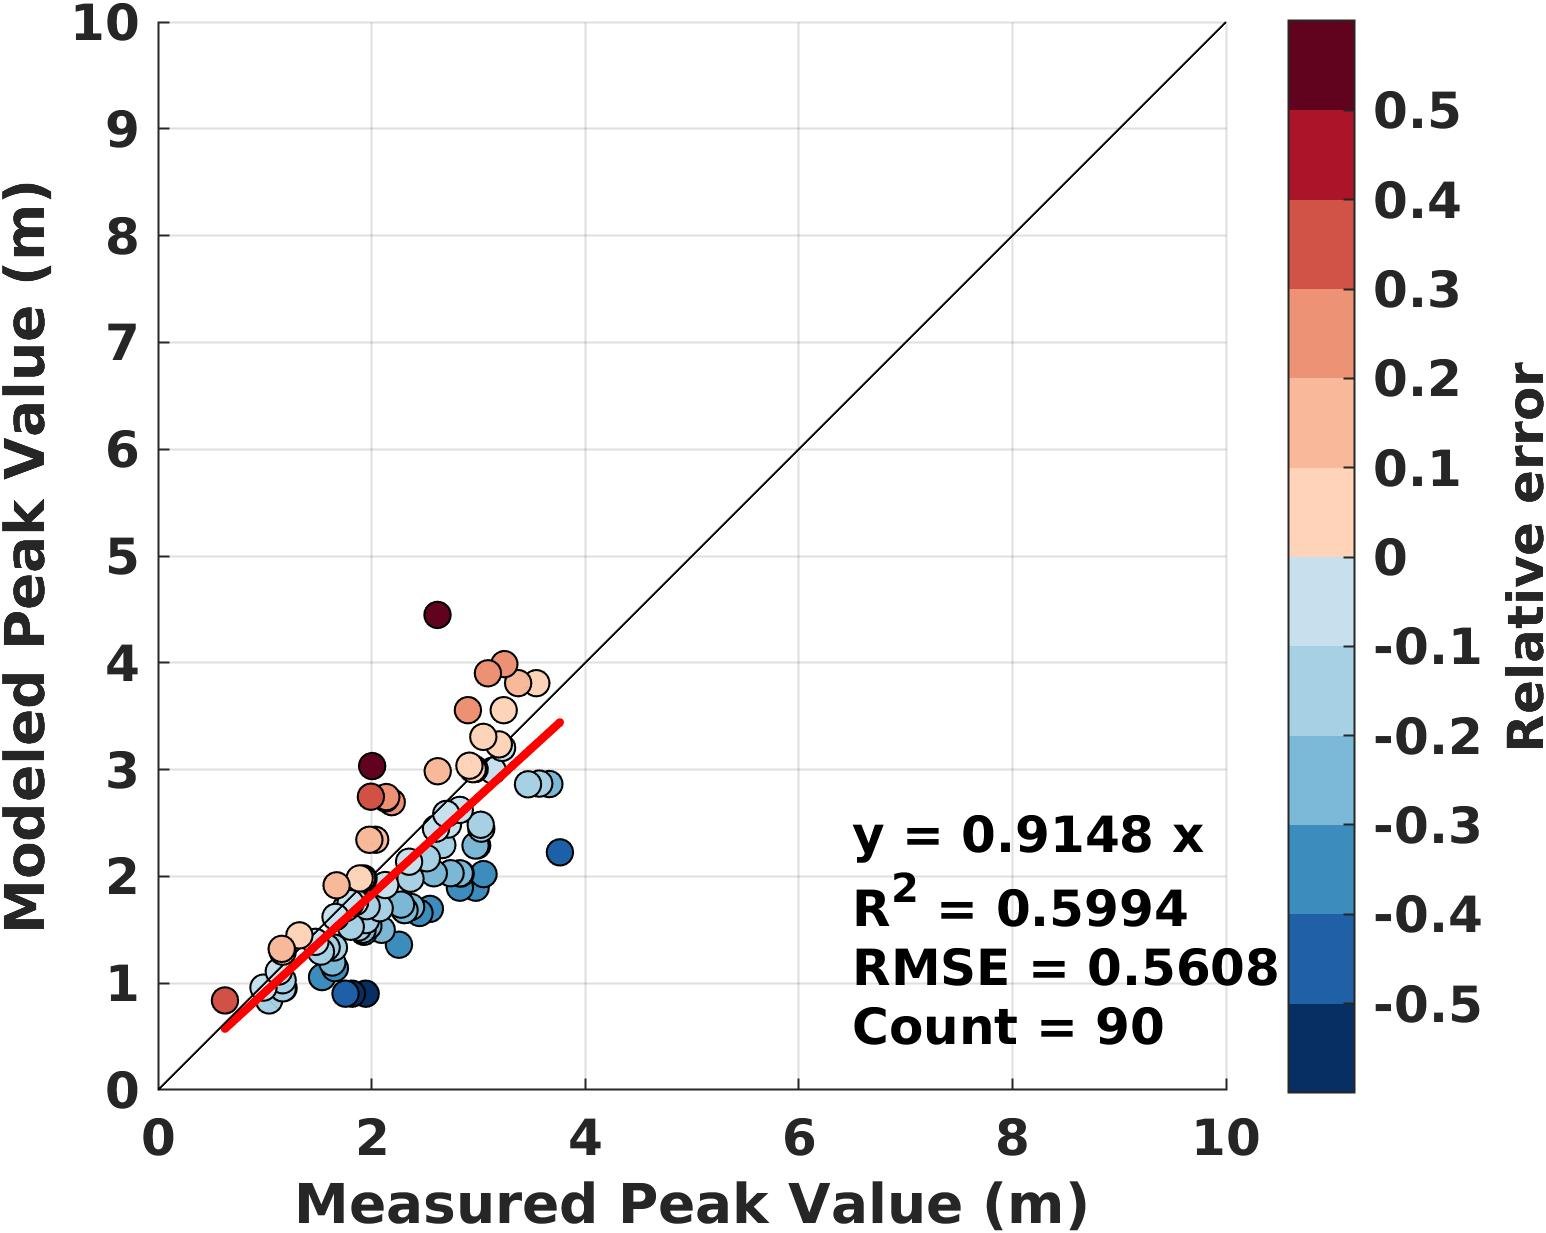
\includegraphics[width=\linewidth]{2008_norain.jpg}

    \column{0.5\linewidth}
    \centering
    \vspace{0.5cm}
    \centering
    DG-SWEM with R-CLIPER
    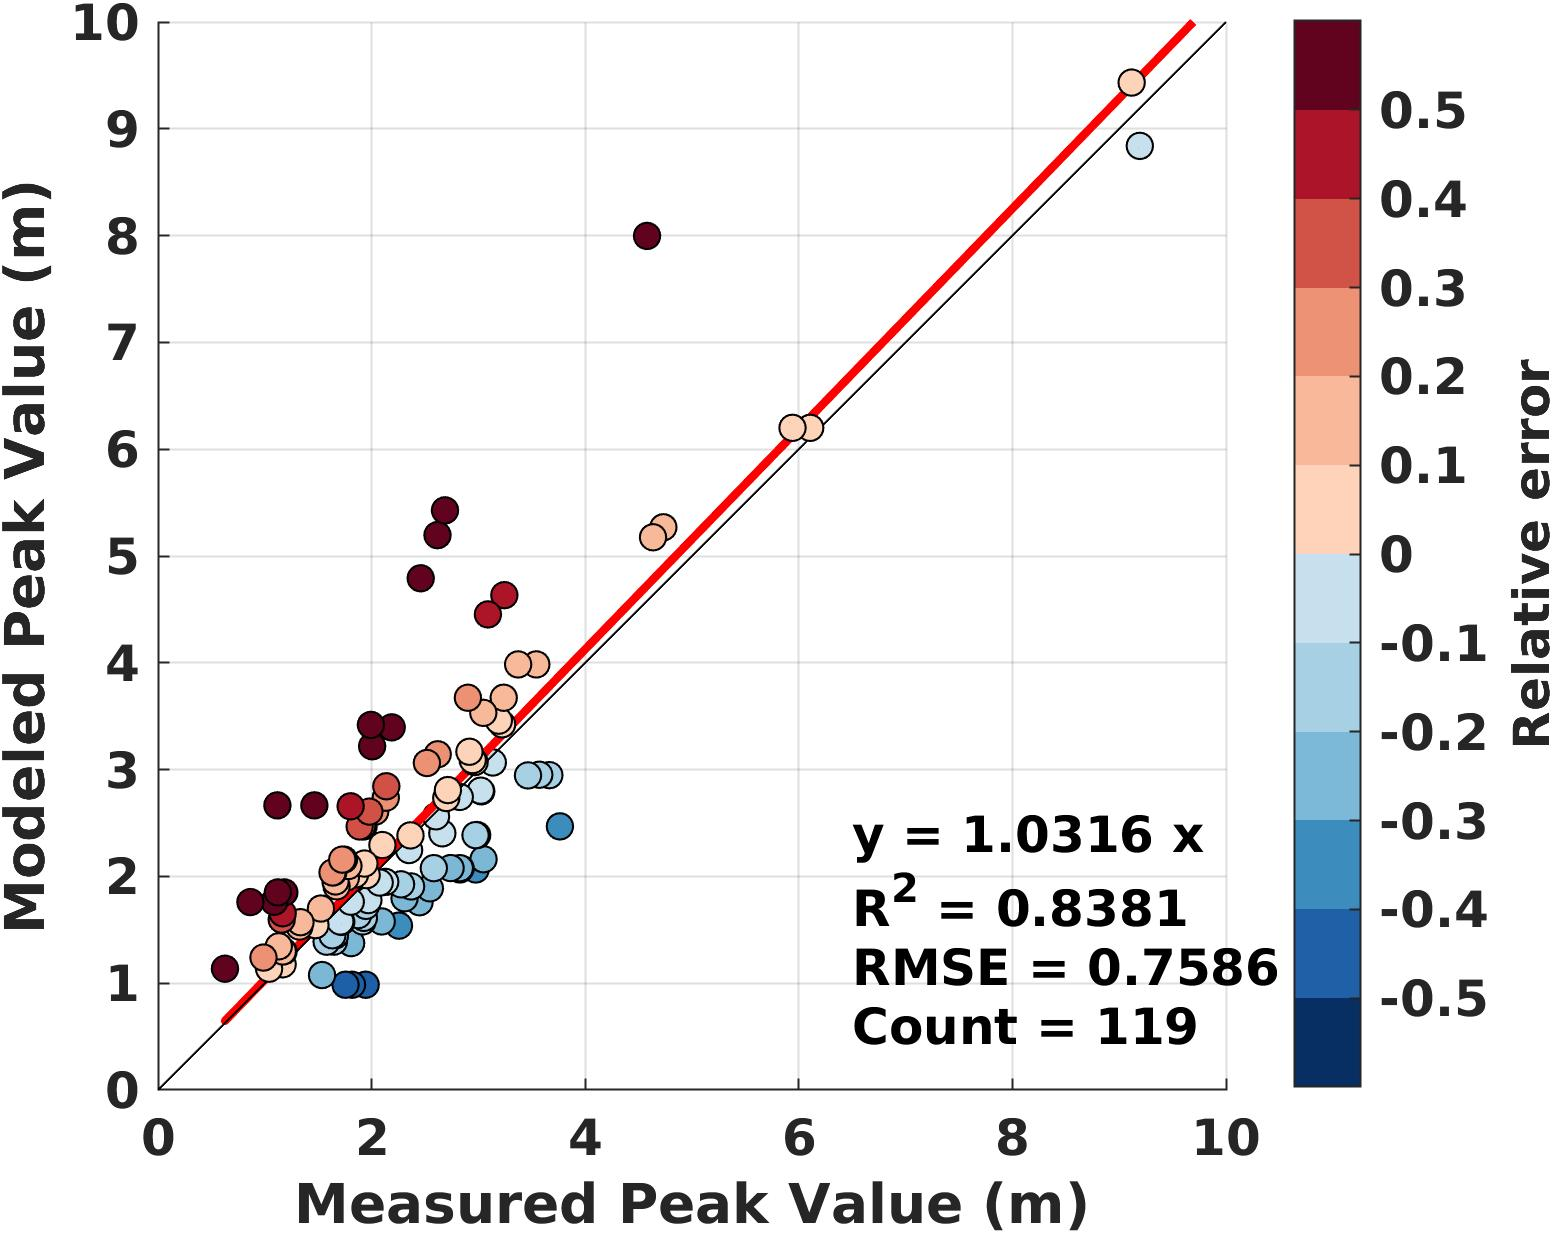
\includegraphics[width=\linewidth]{2008_rain.jpg}

  \end{columns}
\end{frame}

\begin{frame}
  \frametitle{Results - High Water Marks Comparisons}
  \begin{columns}
    \column{0.5\linewidth}
    \centering
    \vspace{0.5cm}
    \centering
    DG-SWEM with observed rain
    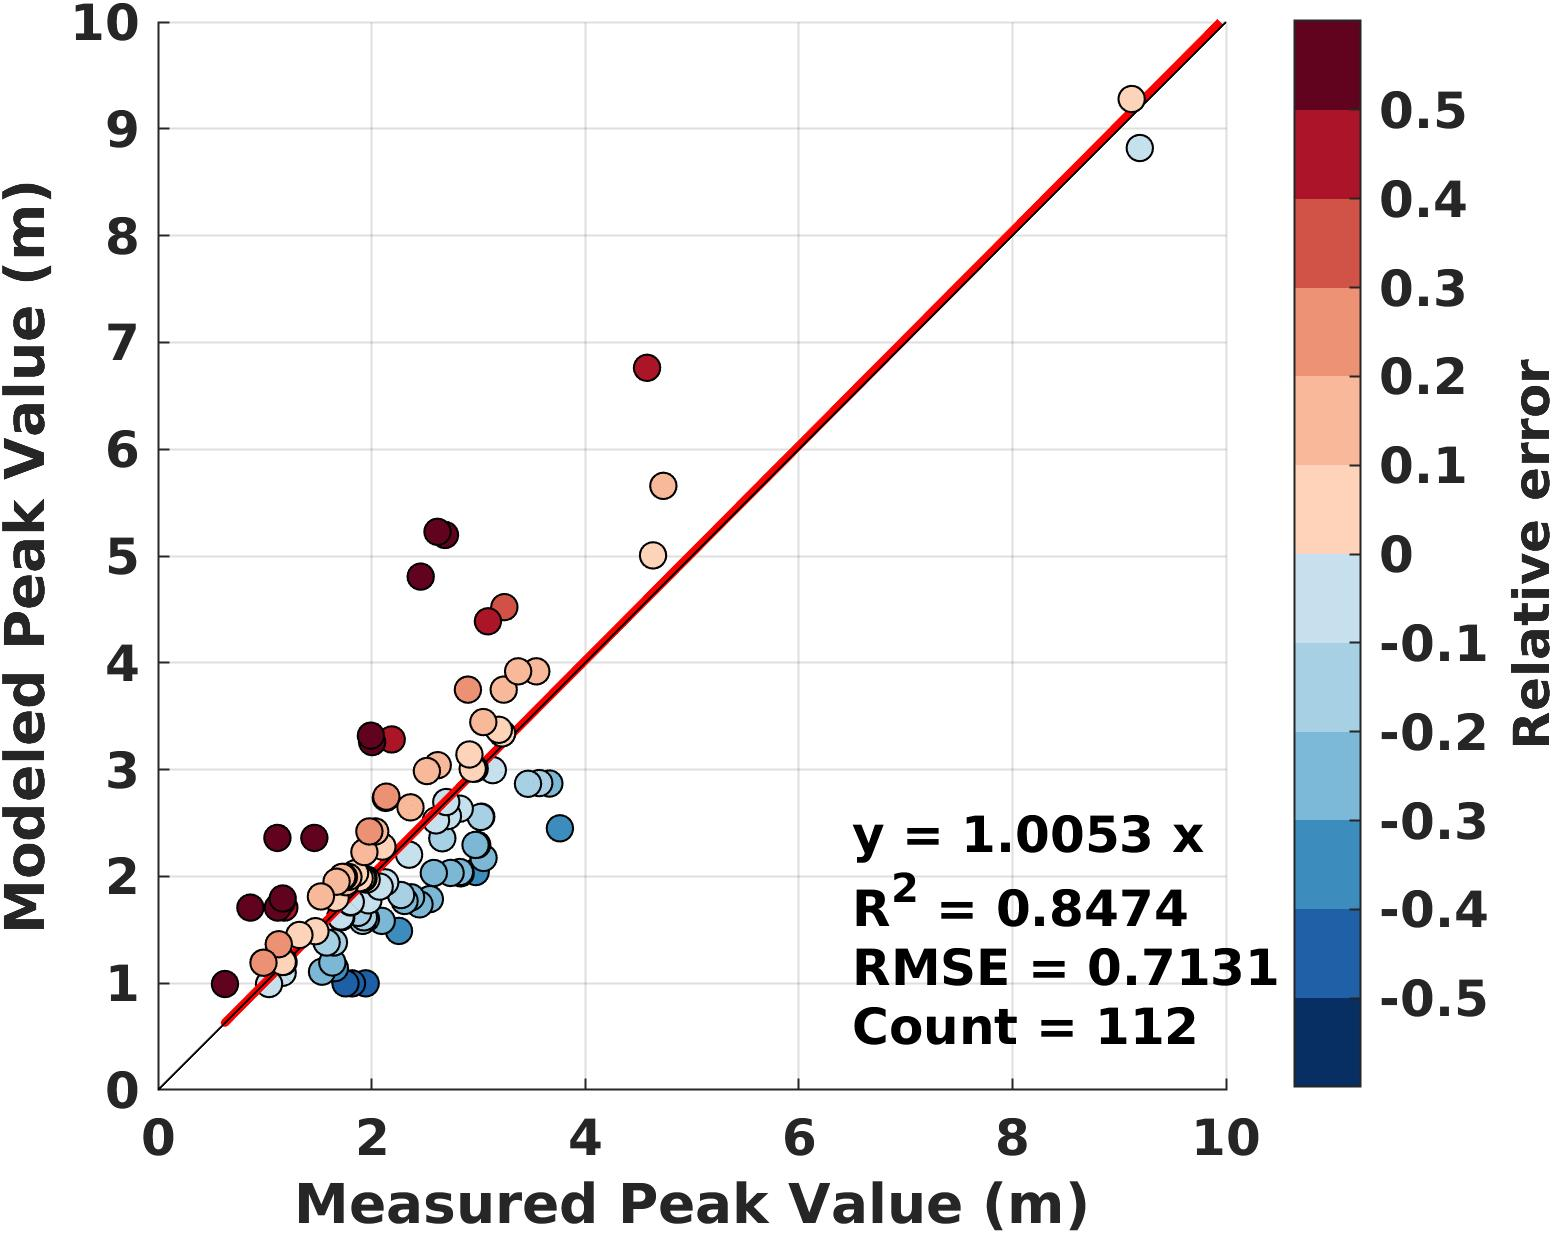
\includegraphics[width=\linewidth]{2008_owi.jpg}

    \column{0.5\linewidth}
    \centering
    \vspace{0.5cm}
    \centering
    DG-SWEM with R-CLIPER
    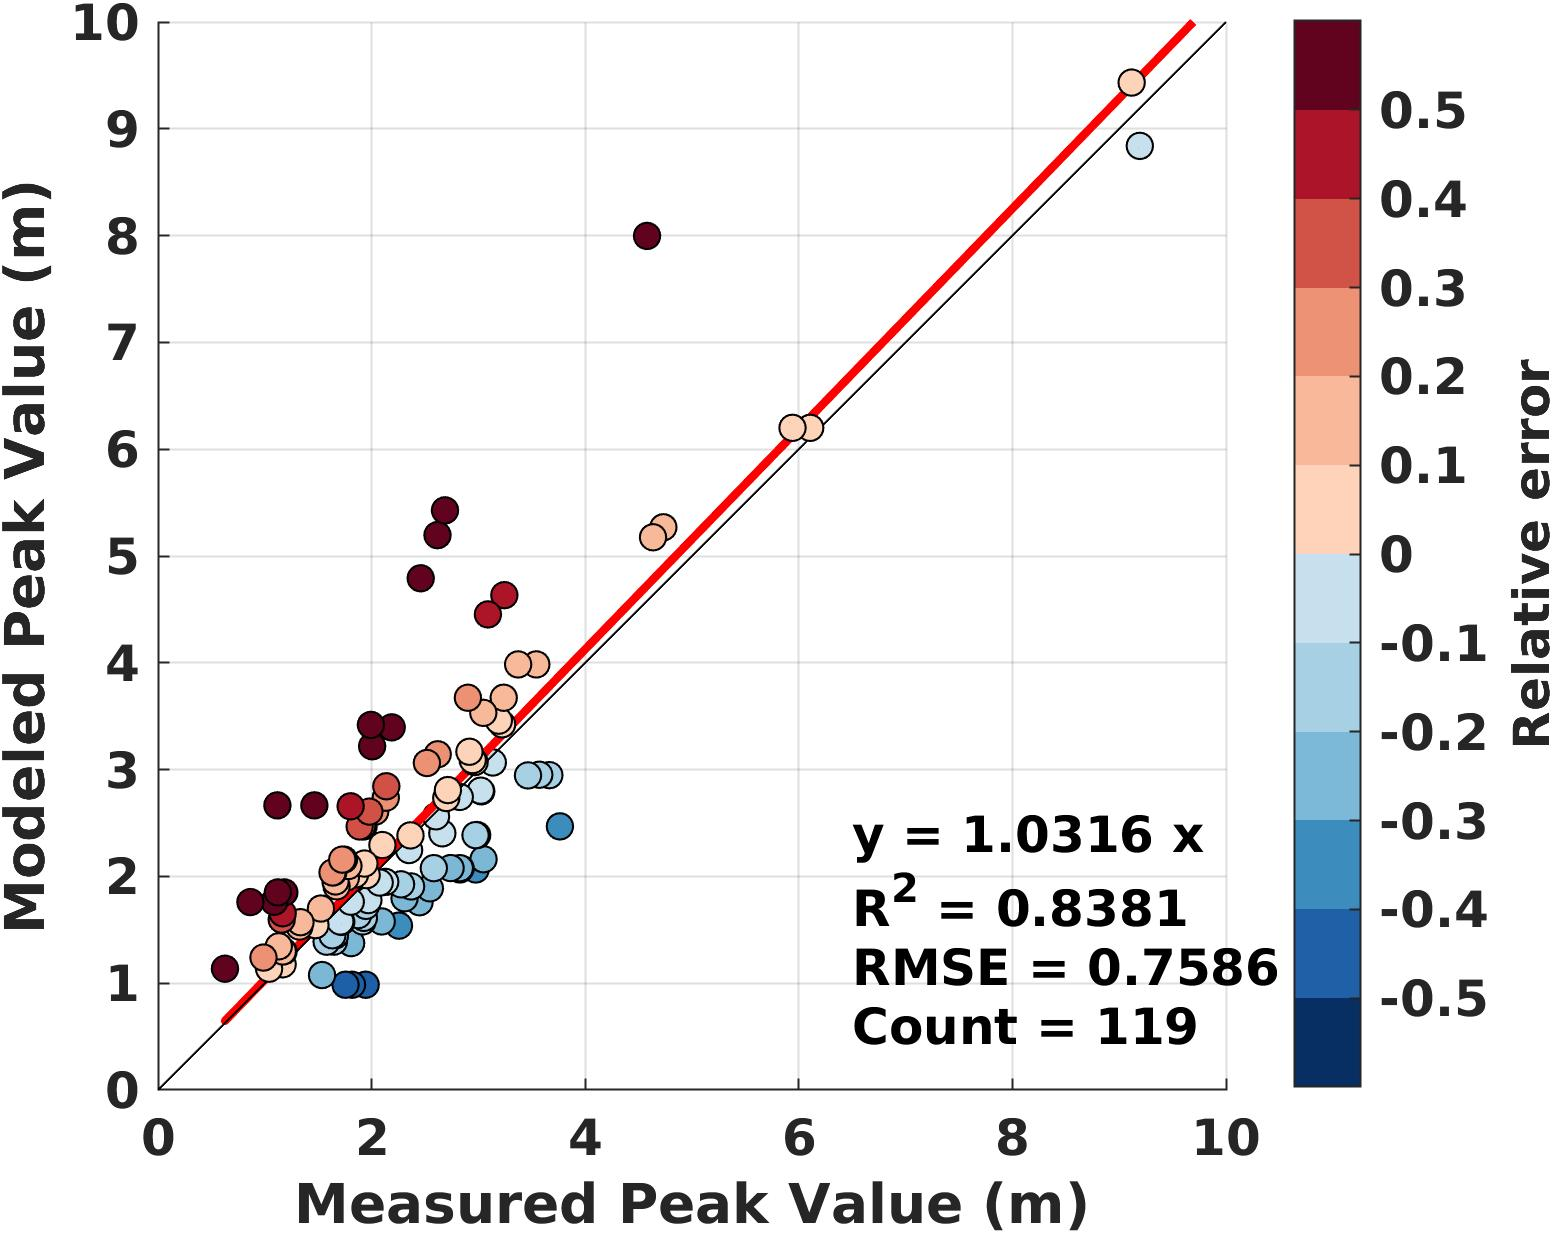
\includegraphics[width=\linewidth]{2008_rain.jpg}

  \end{columns}
\end{frame}
\begin{frame}
  \frametitle{Conclusion and current work}
  \begin{itemize}
  \item Incorportation of rainfall slightly raises overall surface elevation
  \item High water mark comparisons indicate a lot overprediction at certain points by both parametric and observed rain
  \item Underpredictions after peak for locations along the coast; no consistent trend of parametric vs. observed rain
  \end{itemize}
  Work in progress:
  \begin{itemize}
  \item Investigate the spatial distribution of high water marks
  \item Test other parametric rain models (IPET is being incorporated)
  \item Different ways of processing rain data, e.g. interpolation choices, distribution of nodal rain over elements
  \item Test other datasets
  \item Increase DG approximation order to decrease model error
  \end{itemize}
\end{frame}


\end{document}